%*****************************************
\chapter{\textbf{Gaia and SuperWASP sample data}}\label{ch: Data}
%*****************************************

\section{Introduction}

The main goal of the project is to target young-star populations to enhance the probability of observing exoplanetary rings transiting in front of their parent star. Therefore, we mainly focused our study in the well-known OB association Sco-Cen which is mainly sub-divided into three different regions: Lower Centaurus Crux (LCC), Upper Centaurus Lupus (UCL), and Upper Scorpius (US). The \textit{Gaia}-DR1 and-DR2 data were used to select the final sample of stars satisfying conditions on the distance, parallaxes and proper motions based on previous research (\cauthor{2018MNRAS.tmp..210W}\citeyear{2018MNRAS.tmp..210W}; \cauthor{2016MNRAS.461..794P}\citeyear{2016MNRAS.461..794P}; \cauthor{1989A&A...216...44D}\citeyear{1989A&A...216...44D}). However, also a selection based on stellar evolution tracks and isochrones using the \textit{MESA}-code provided through the \textit{MIST}-package (\cauthor{2016ApJS..222....8D}\citeyear{2016ApJS..222....8D}; \cauthor{2016ApJ...823..102C}\citeyear{2016ApJ...823..102C}) was performed to guarantee that the final sample consists of stars between $5$Myr to $60$Myr. This informations is needed in order to obtain the $RA$ and $DEC$ coordinates of the objects of interest and retrieve the available light curves using the \textit{SuperWASP}-database (\cauthor{2010A&A...520L..10B}\citeyear{2010A&A...520L..10B}). The main results from the \textit{Gaia}-and \textit{SuperWASP}-queries are presented in more detail the next sections, including the light-curves preliminary results which are addressed extensively in \autoref{ch: Results} .   
%============================================================================================================================================================

\section{Sco-Cen OB Association}
%============================================================================================================================================================

\section{Gaia Samples}

The \textit{Gaia}-DR1 and-DR2 data was used to select stars which belong to the Sco-Cen OB association. The queries were carried out using the ADQL-query interface provided by the ESA (\url{https://gea.esac.esa.int/archive/}) and shown in \autoref{ch:Appendix} for each of the three regions conforming Sco-Cen i.e. LCC, UCL, and US. The approach was tested in \textit{Gaia}-DR1, but later on was extended to the new data provided by the DR2 to increase the sample of stars belonging to Sco-Cen, and also to increase the chance of matching a star with a light curve in the \textit{SuperWASP}-database. This will be addressed at the end. The most relevant parameters retrieved for each object are the RA and DEC coordinates, galactic longitude (l) and latitude (b), parallax, magnitude in the G-band, color G-Ks, and the proper motion in RA and DEC.\\    

First of all, a sample based on previous physical parameters and values obtained for this association is needed in order to constrain the sample and avoid pollution from stars which may not be part of it. Following \cauthor{2018MNRAS.tmp..210W}\citeyear{2018MNRAS.tmp..210W}, the spatial distribution of the three regions were selected using the galactic coordinates cut reported by \cauthor{2012yCat..74163108R}\citeyear{2012yCat..74163108R} and \cauthor{1999AJ....117..354D}\citeyear{1999AJ....117..354D} as shown in \autoref{tab:ScoCen_SpatialDist}. Also in distance, using a parallax range from $6$mas to $12$mas which leads to a distance range of $\sim 83-167$pc. We decided to include a wide range in distance because Sco-Cen spanning distances are known to be $\sim 100-150$pc \cauthor{2018MNRAS.tmp..210W}\citeyear{2018MNRAS.tmp..210W}, so we can rule out any outliers based on the dynamics of the cluster. The spatial distribution of our sample is shown in \autoref{fig:Projection_ScoCen}. The blue, orange, and red dots represent LCC, UCL, and US respectively. It is clear that the Sco-Cen association covers a wide range in galactic longitude (l) $\sim 90$-deg, and $\sim 45$-deg in galactic latitude (b). Following this, initially each sub-region contains LCC $= 2310$, UCL $= 1759$, and US $= 1584$ stars respectively. However, as it is mentioned in \cauthor{2016MNRAS.461..794P}\citeyear{2016MNRAS.461..794P}, each region has a characteristic range for the proper motions given by the dynamics of each individual subgroup and the whole interaction. According tho their work, the three subgroups have a value of $\mu_\alpha < 10~\textnormal{mas}~\textnormal{yr}^{-1}$ and $\mu_\delta = 30~\textnormal{mas}~\textnormal{yr}^{-1}$, while for LCC, UCL, and US values of $15~\textnormal{mas}~\textnormal{yr}^{-1} < \mu < 55~\textnormal{mas}~\textnormal{yr}^{-1}$, $12~\textnormal{mas}~\textnormal{yr}^{-1} < \mu < 55~\textnormal{mas}~\textnormal{yr}^{-1}$, and $\mu < 47~\textnormal{mas}~\textnormal{yr}^{-1}$, respectively, are reported. This is better seen in \autoref{fig:Hist_ScoCen_Mamajek} where the histogram for the whole sample of stars selected in distance range are shown in colors, and each vertical dashed-line shows the above mentioned cuts for each subgroup. In the end, after this analysis, the query was performed taking into account the dynamical constraints of the cluster (see \autoref{ch:Appendix}).\\  

\begin{table}[]
\centering
\caption{\scriptsize{Something!}}
\label{tab:ScoCen_SpatialDist}
\begin{tabular}{lcccc}
\hline
Sub-group             & l$_{-}$ {[}deg{]} & l$_{+}$ {[}deg{]} & b$_{-}$ {[}deg{]} & b$_{+}$ {[}deg{]} \\ \hline \hline
Lower Centaurus Crux  & 285               & 313               & -10               & 16                \\
Upper Centaurus Lupus & 313               & 337               & 5                 & 31                \\
Upper Scorpius        & 337               & 360               & 7                 & 32                \\ \hline \hline
\end{tabular}
\end{table}

\begin{figure}[!ht]%
    \centering
    \subfloat{{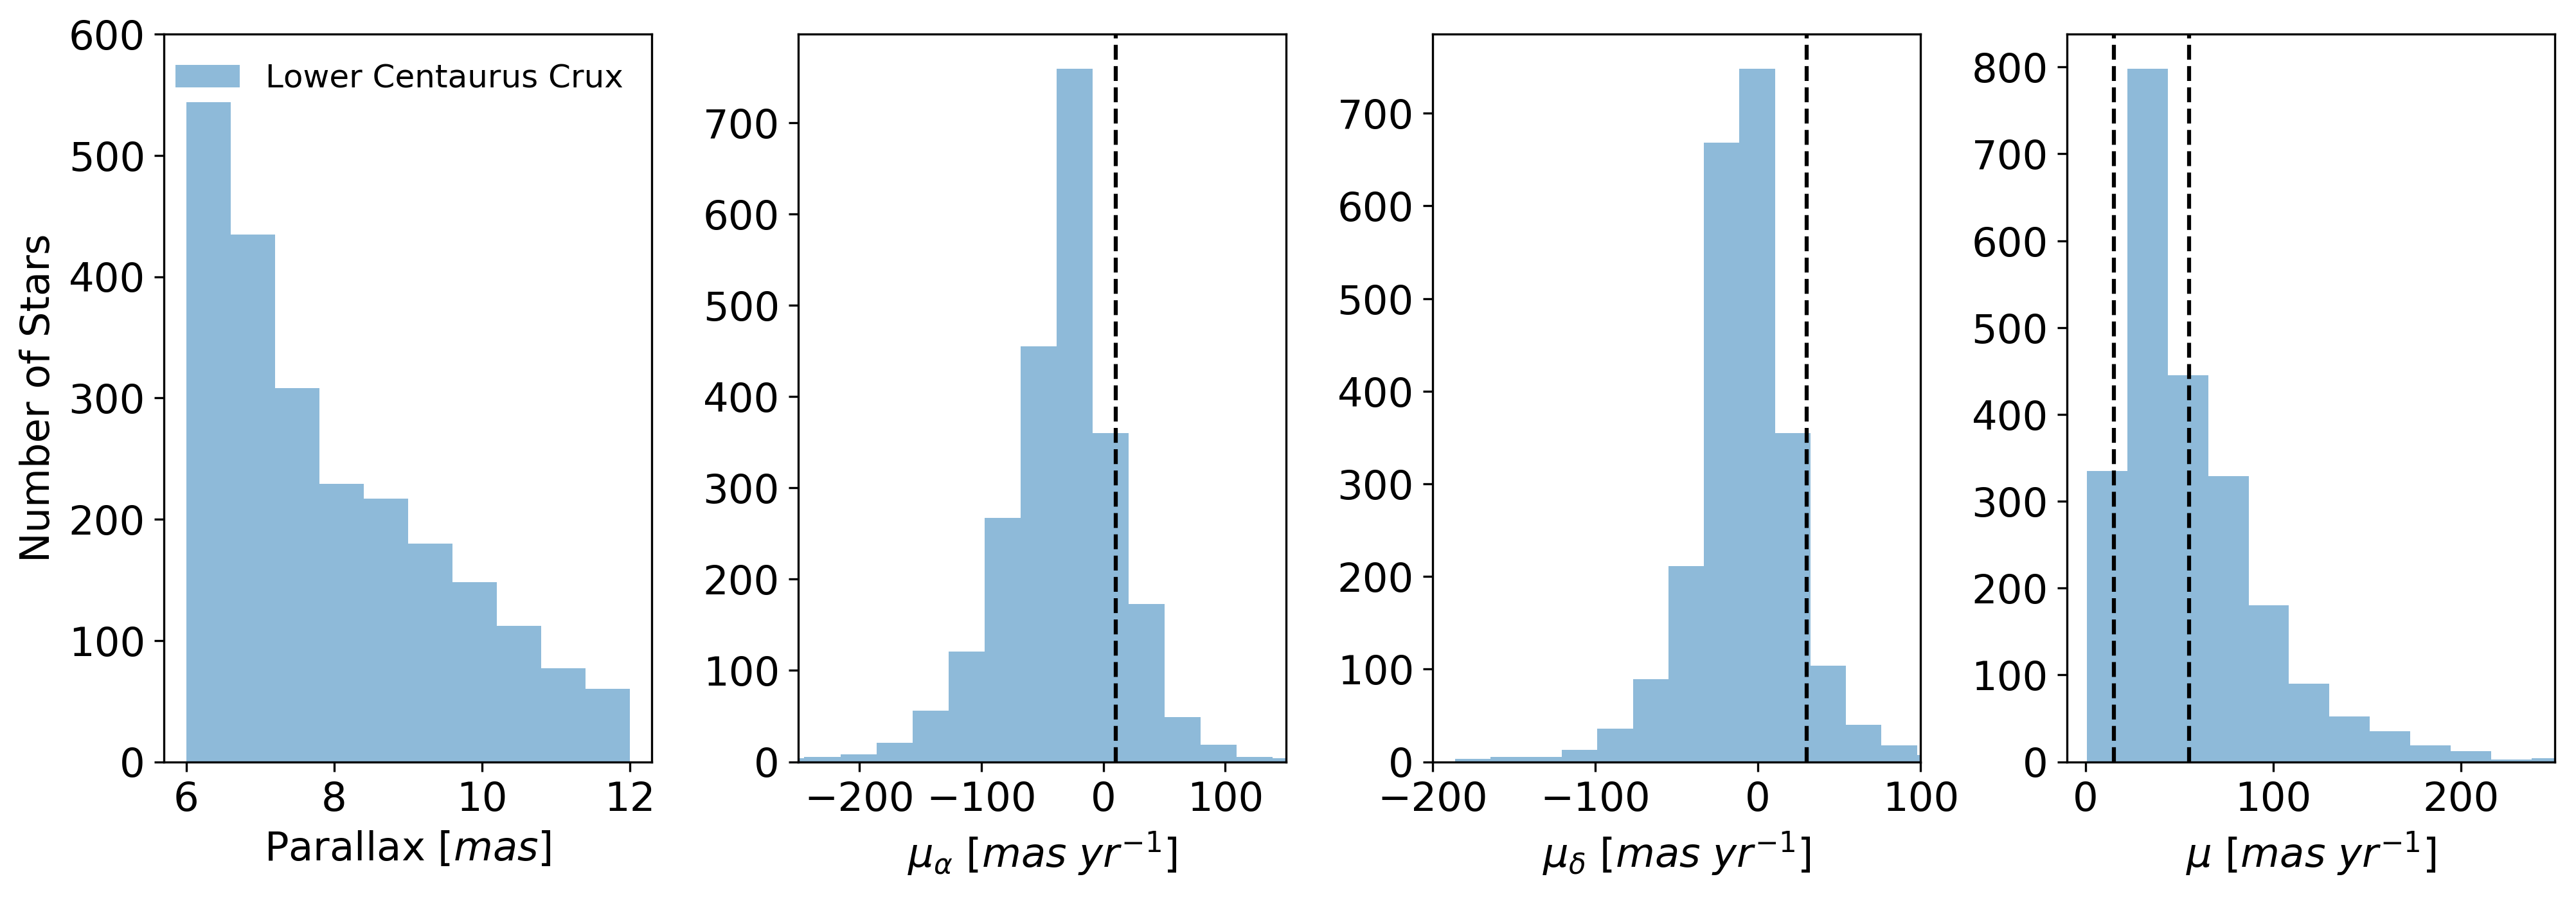
\includegraphics[width = 16cm, height = 5.5cm]{./Graficos/Capitulo_3/5_Sco-Cen/Hist_Extintion_1.png} }}%
    \qquad
    \subfloat{{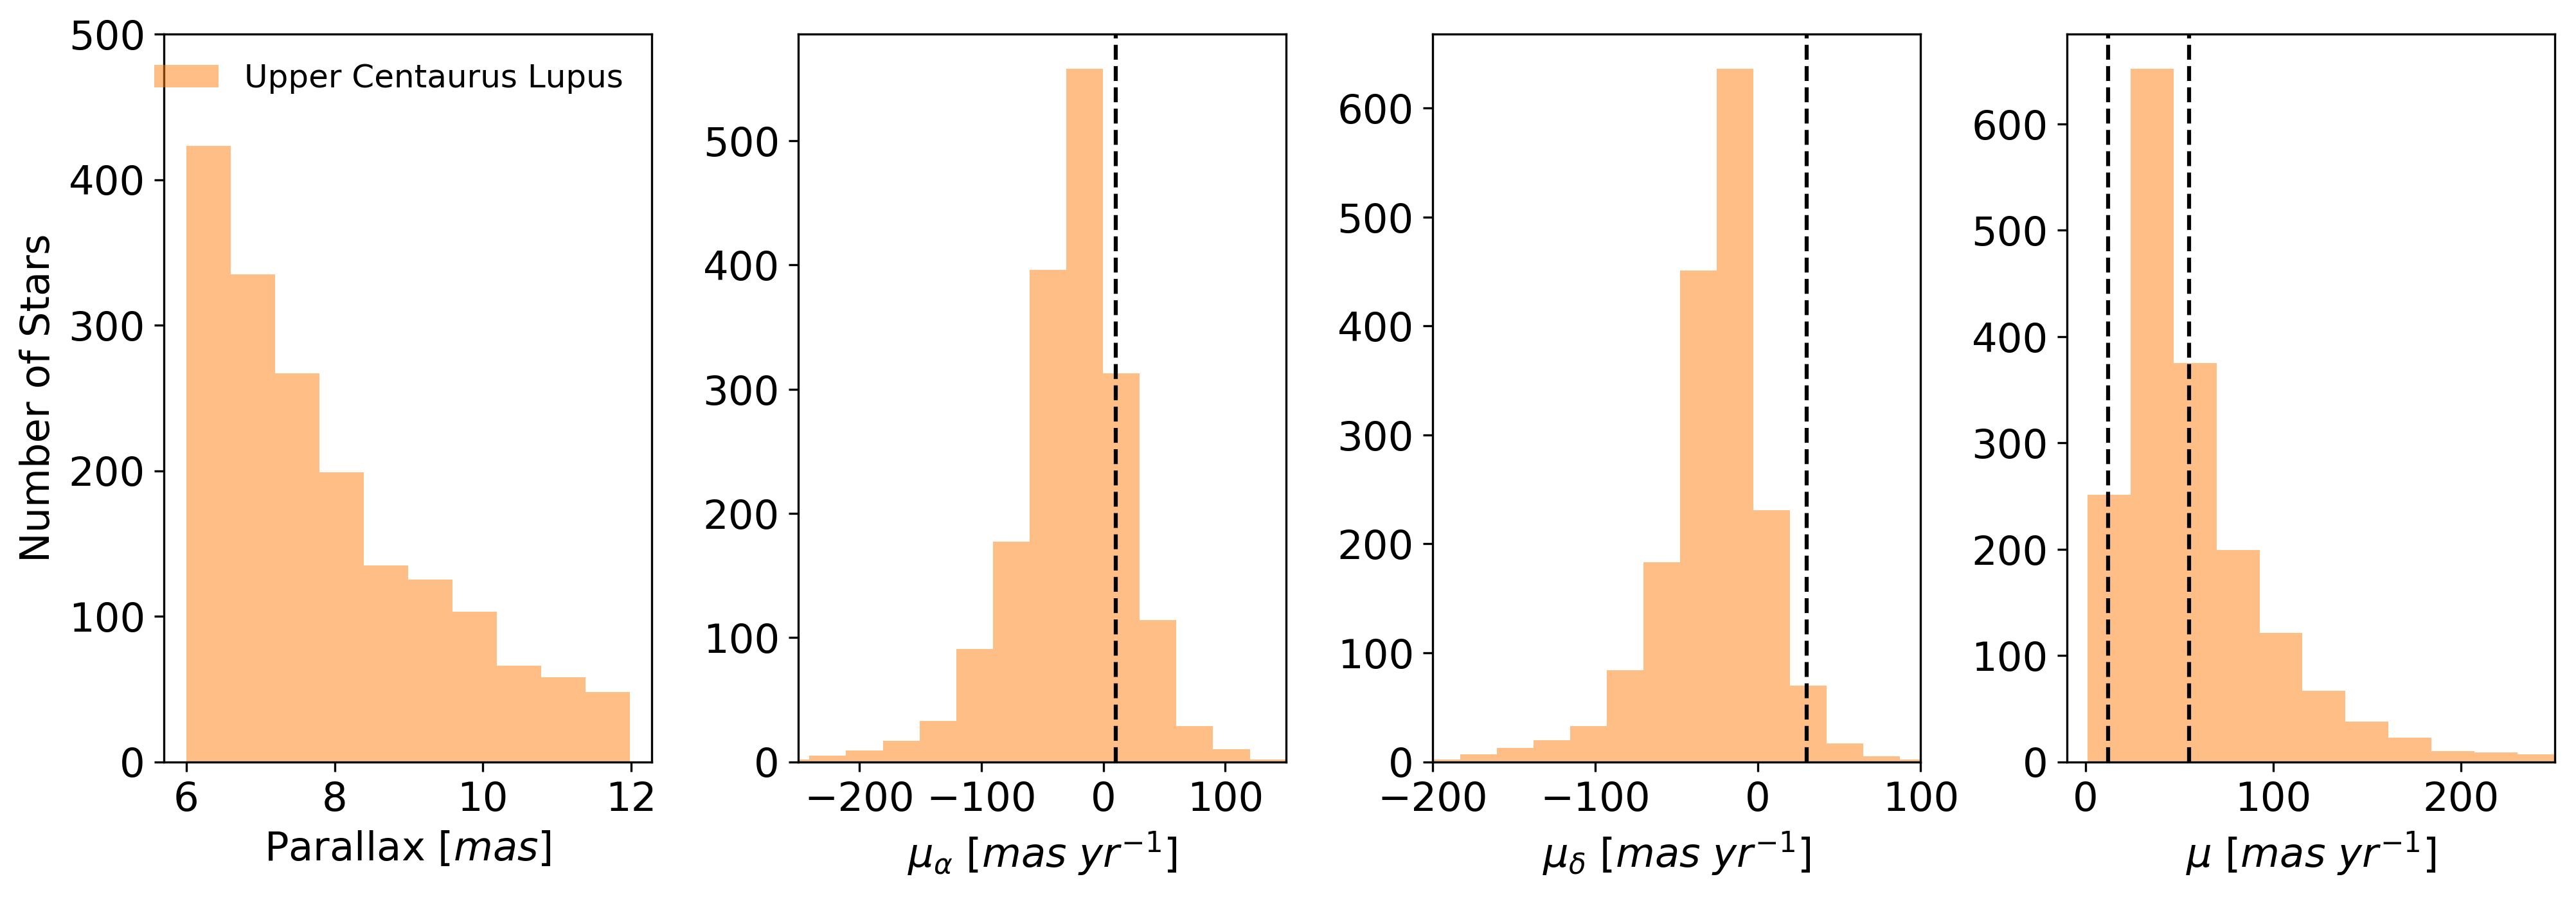
\includegraphics[width = 16cm, height = 5.5cm]{./Graficos/Capitulo_3/5_Sco-Cen/Hist_Extintion_2.png} }}%
    \qquad
    \subfloat{{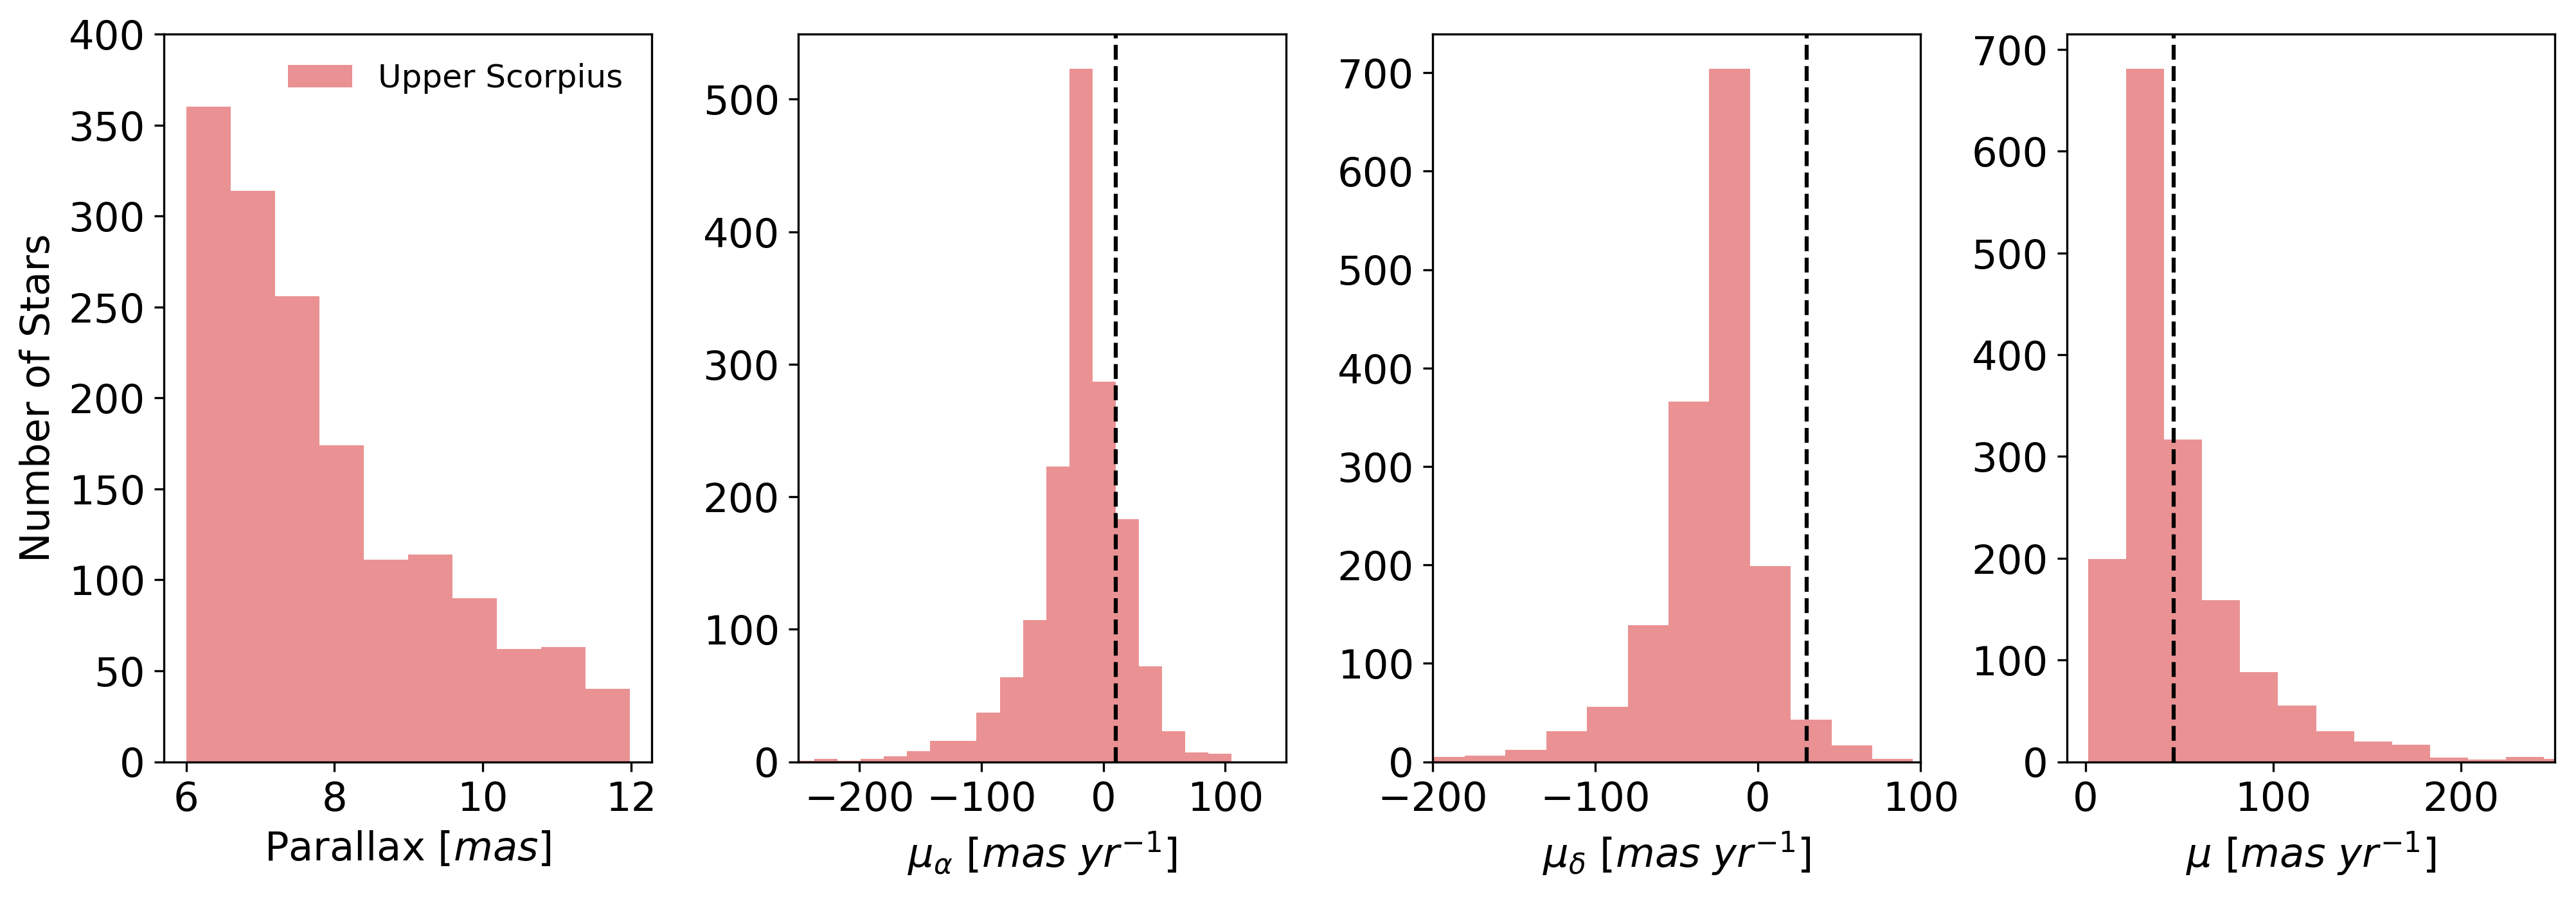
\includegraphics[width = 16cm, height = 5.5cm]{./Graficos/Capitulo_3/5_Sco-Cen/Hist_Extintion_3.png} }}%
    \caption{\scriptsize{Something!}}%
    \label{fig:Hist_ScoCen_Mamajek}%
\end{figure}  

\begin{figure}[!ht]
\centering
  \subfloat{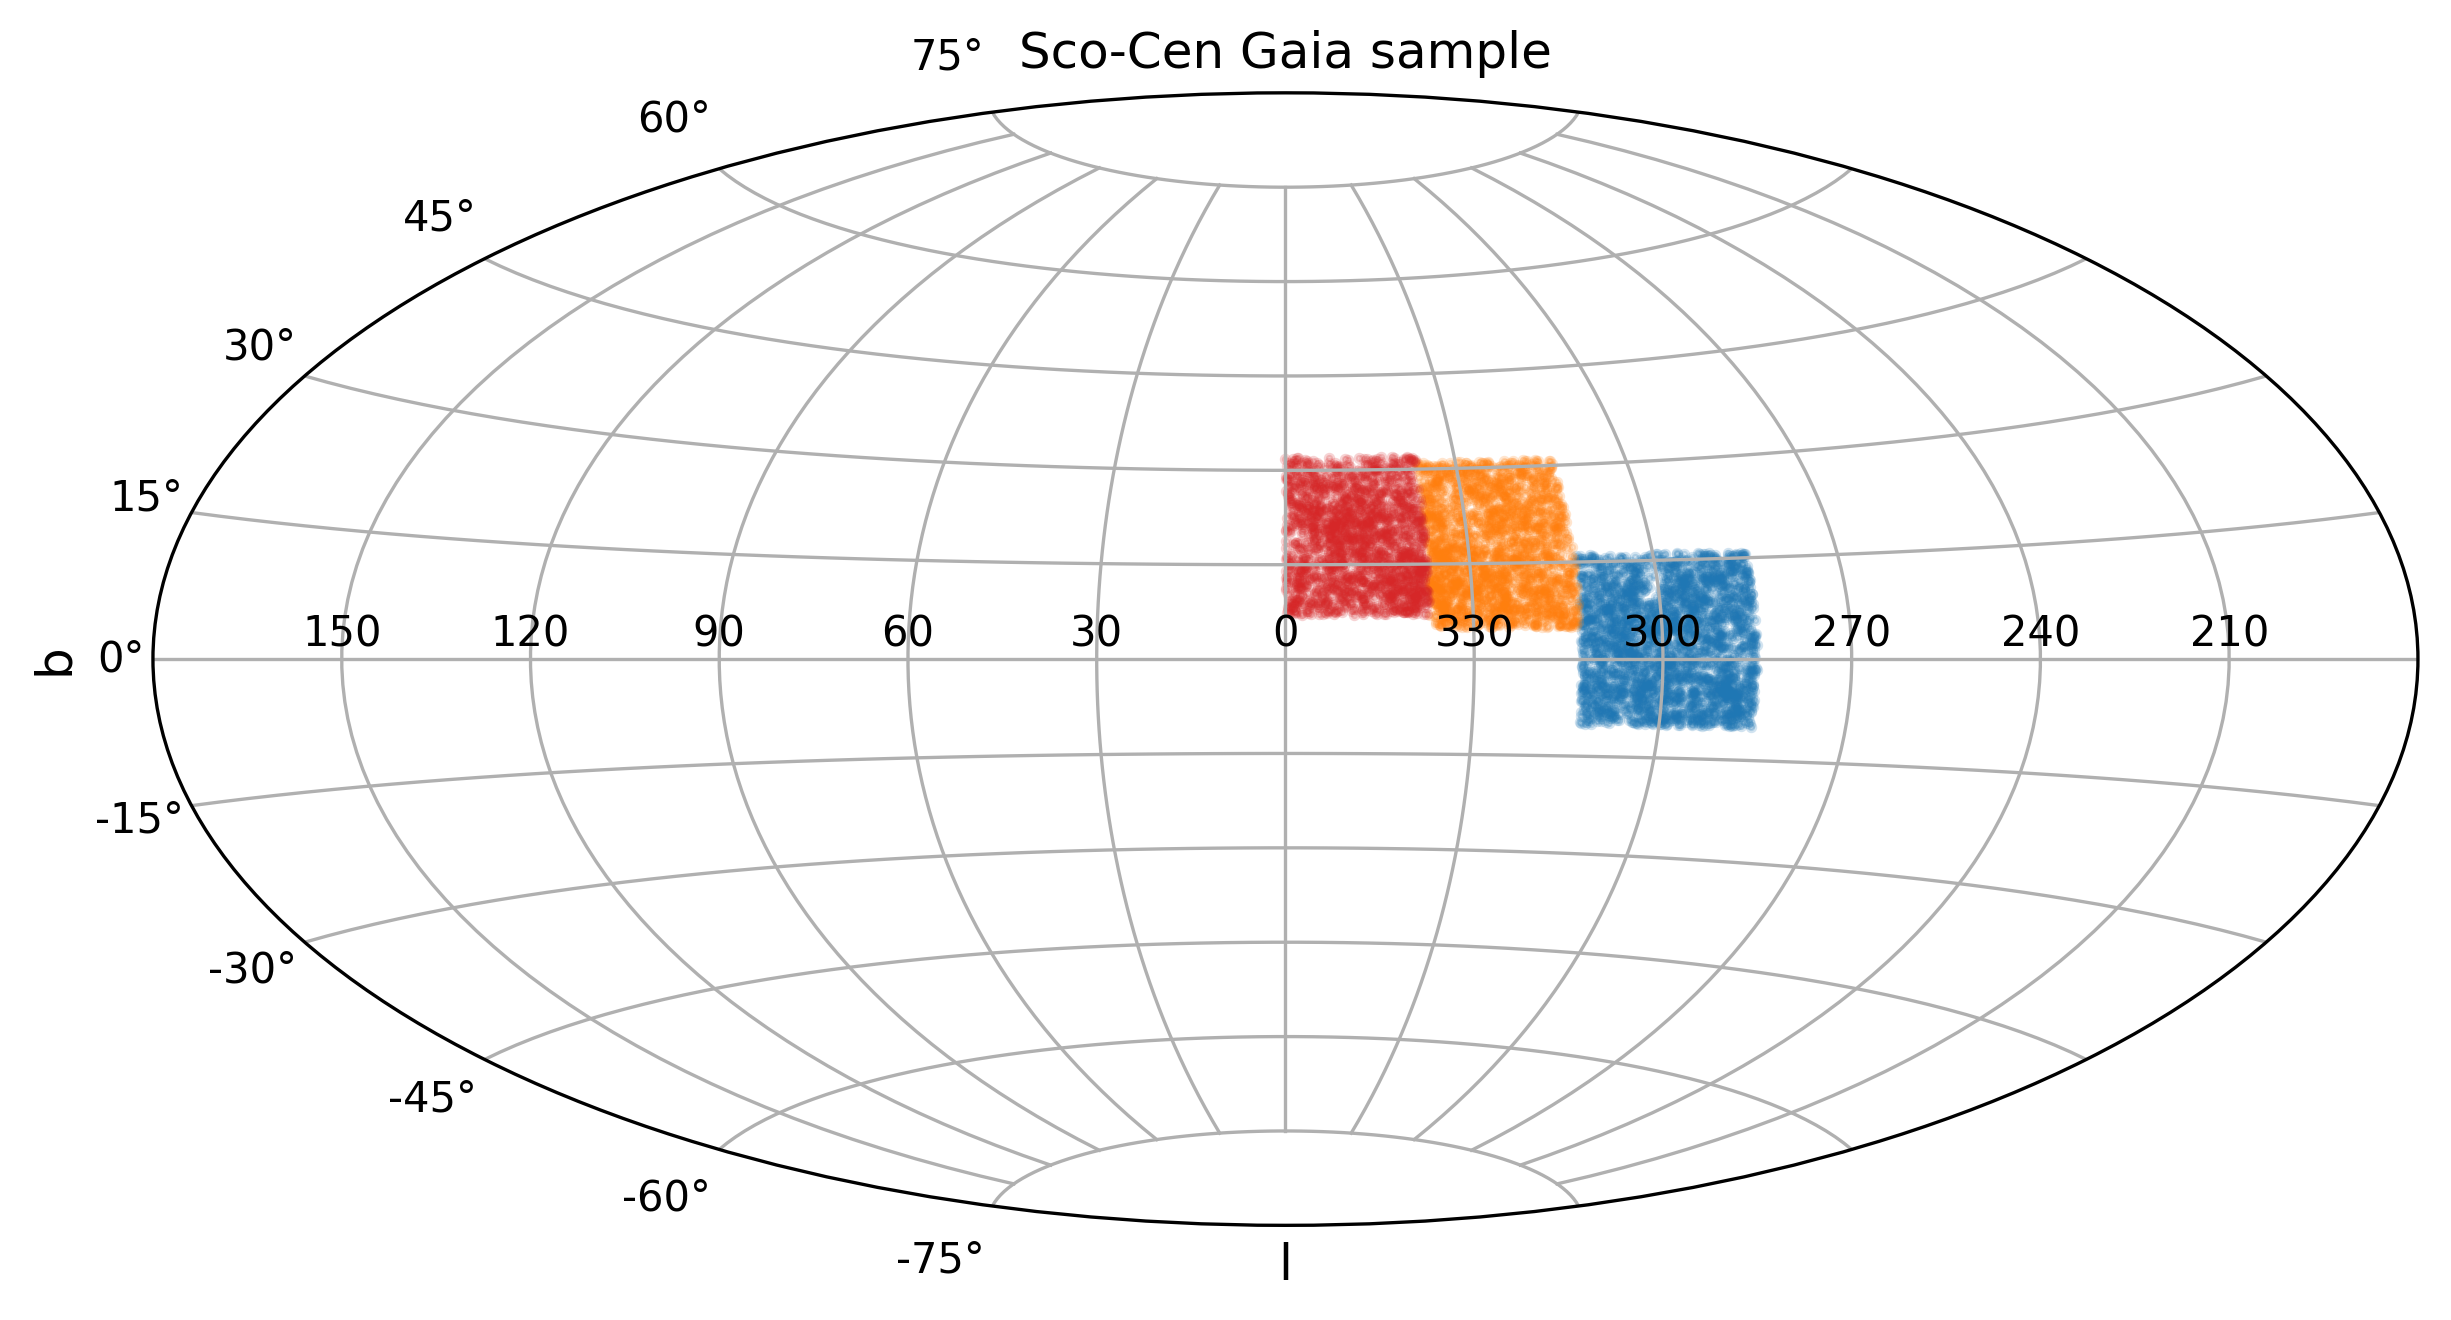
\includegraphics[width = 12cm, height = 7cm]{./Graficos/Capitulo_3/5_Sco-Cen/Sco_Cen_Projection_flipped.png}} 
\caption{\scriptsize{Something!}}
\label{fig:Projection_ScoCen}
\end{figure}

This cut-off in proper motion and parallax leads to a new sample of LCC $= 1010$, UCL $= 746$, and US $= 797$ stars respectively, in which we have ruled out stars which certainly do not belong to the association. The next step is to narrow down the sample based on the stellar evolution of the cluster. This was performed using evolutionary tracks in which we aimed to use low mass stars as they are the ones with higher probabilities of exo-ring transits as shown before, and also using isochrones to restrict each sample in stellar age. This is thoroughly explained in \autoref{sec:SEM_1}.   


%============================================================================================================================================================

\section{Stellar Evolution Models}\label{sec:SEM_1}

The highest transit probability was obtained for low mass stars. As shown in \autoref{fig:Rings_Prob}, the probability of detecting rings transiting in front of the parent stars decreases as the stellar mass increases independent of the life time for the planetary rings which only causes a vertical shift i.e. a chance in the expected number of transits. Therefore, it is important to select a reliable sample of stars in Sco-Cen which can lead to a high chance of detecting this kind of transits. The first step consisted in taking the sample mentioned above in which a cut-off in the dynamics and distance for the association has been applied, and run different stellar track models with an initial value of extinction $\textnormal{A}_\textnormal{v} = 0$ for each sub-region using the \textit{MIST}-package. In \autoref{fig:Stellar_Tracks_1}, the color-magnitude diagram for each sub-region is presented for $\textnormal{G}$- and $\textnormal{K}_\textnormal{s}$-bands. The magnitudes were obtained using \textit{Gaia}-DR1 and transformed to absolute magnitude (see \autoref{ch:Appendix}). The color was computed using a cross-match identification of the sources in \textit{Gaia}-DR1 with \textit{The Two Micron All-Sky Survey} (2MASS) tables. The stellar tracks shown correspond to stellar masses from $0.5 \textnormal{M}_\odot$ to  $2.1 \textnormal{M}_\odot$ in steps of $0.4 \textnormal{M}_\odot$, which were computed for the required photometric bands in \textit{Gaia} and \textit{2MASS}. Although each sub-region shows different spread, the stars seem to be distributed mostly below the $1.3 \textnormal{M}_\odot$ stellar track. Therefore, no-extra cut-off in mass in needed because if one compares to \autoref{fig:Rings_Prob} the highest probabilities lie below $2.0 \textnormal{M}_\odot$. The same conditions were assumed to compute the isochrones shown in \autoref{fig:Isochrones_1}. Each figure corresponds to the LCC, UCL, and US color-magnitude diagrams with isochrones of $5, 15, 20, 30$- and $60$-Myr. The upper isochrone, is the youngest ($5$-Myr) while the lower represents the oldest ($60$-Myr). In each of the three cases, most of the stars are contained in between the youngest and the oldest isochrones. It is useful to have in mind that all the isochrones are computed without extinction factor which is the ideal scenario. A few stars lie outside the isochrones delimited region, thus, the idea is to use the isochrones and only use those stars that satisfy the absolute magnitude $\textnormal{M}_\textnormal{G}$ and color $\textnormal{G} - \textnormal{K}_\textnormal{s}$ conditions in between both isochrones. After obtaining only those stars in between the isochrones the final sample is reduced to LCC $= 868$, UCL $= 633$, and US $= 649$ stars respectively. This is shown in \autoref{fig:Isochrones_2} where one can observe how the initial distribution of stars is already contained in a region delimited by the isochrones. For comparison in \autoref{ch:Appendix}, \autoref{sec:Sample_Selection_1}, it is shown the original sample of stars without performing the proper motion and parallax cut-off in color versus the sample after using \cauthor{2016MNRAS.461..794P}\citeyear{2016MNRAS.461..794P} constraints in black-dots for each sub-region in \autoref{fig:Stellar_Tracks_1_appendix} and \autoref{fig:Isochrones_1_appendix}.\\       

\begin{figure}[!ht]
\centering
  \subfloat{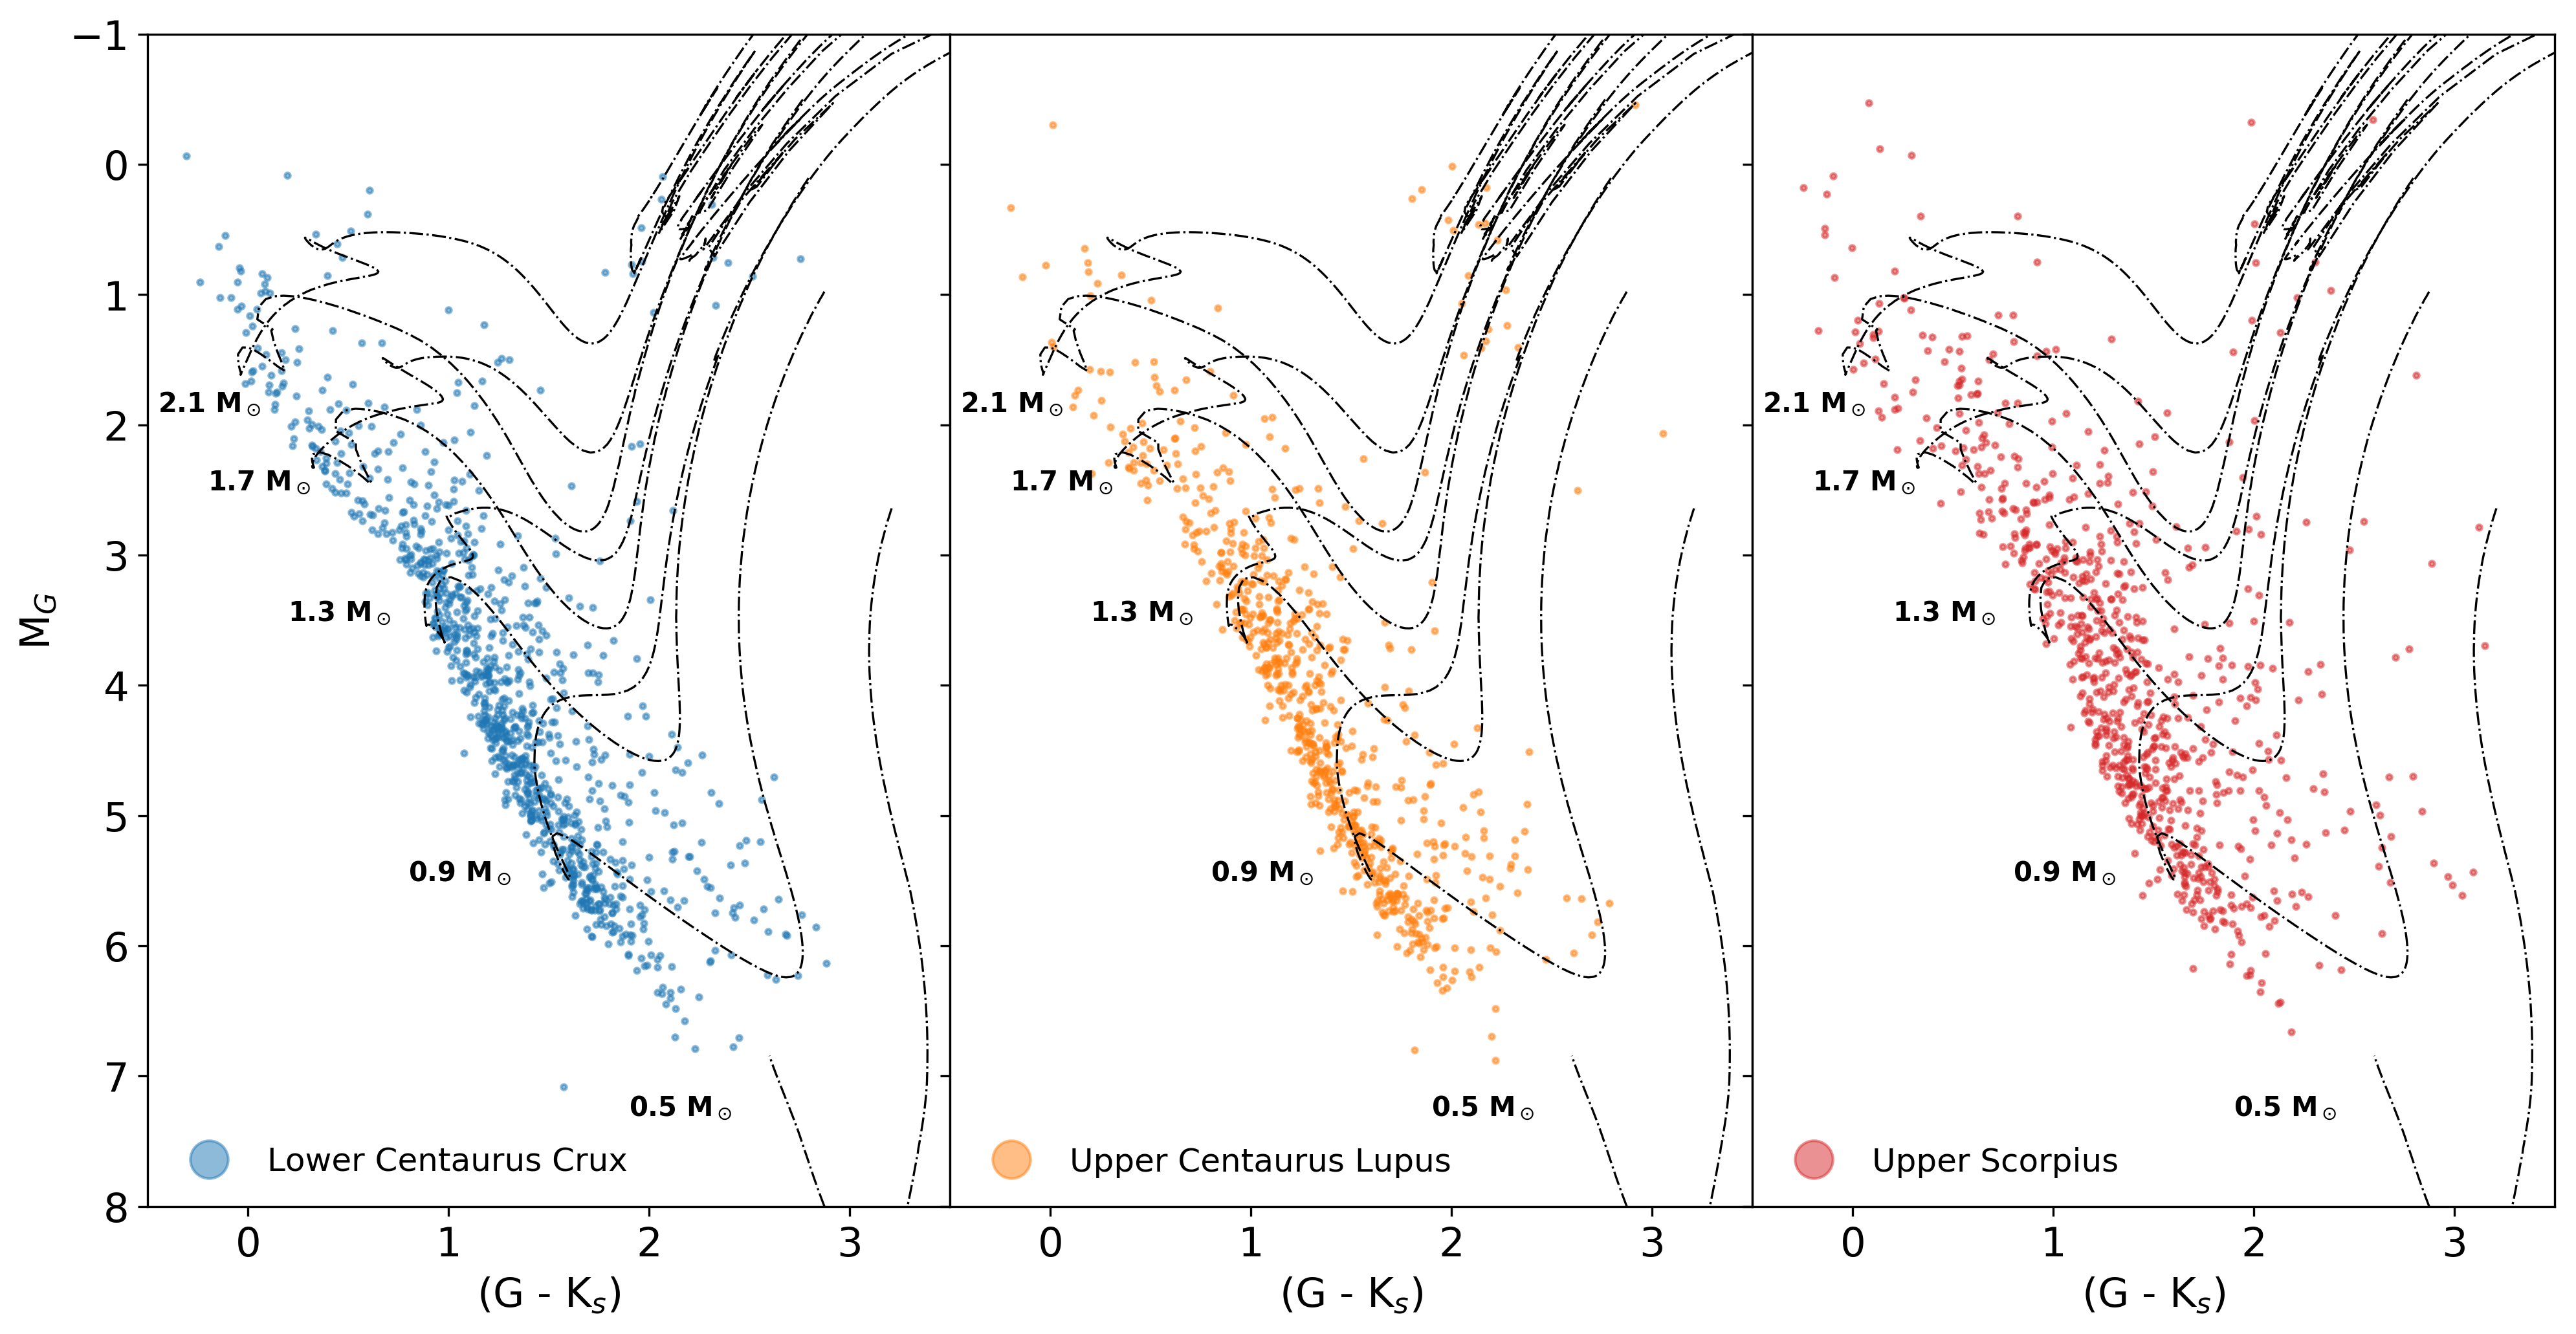
\includegraphics[width = 15cm, height = 8.5cm]{./Graficos/Capitulo_3/5_Sco-Cen/Mag_Col_diagram_4_2.png}} 
\caption{\scriptsize{Something!}}
\label{fig:Stellar_Tracks_1}
\end{figure}

\begin{figure}[!ht]
\centering
  \subfloat{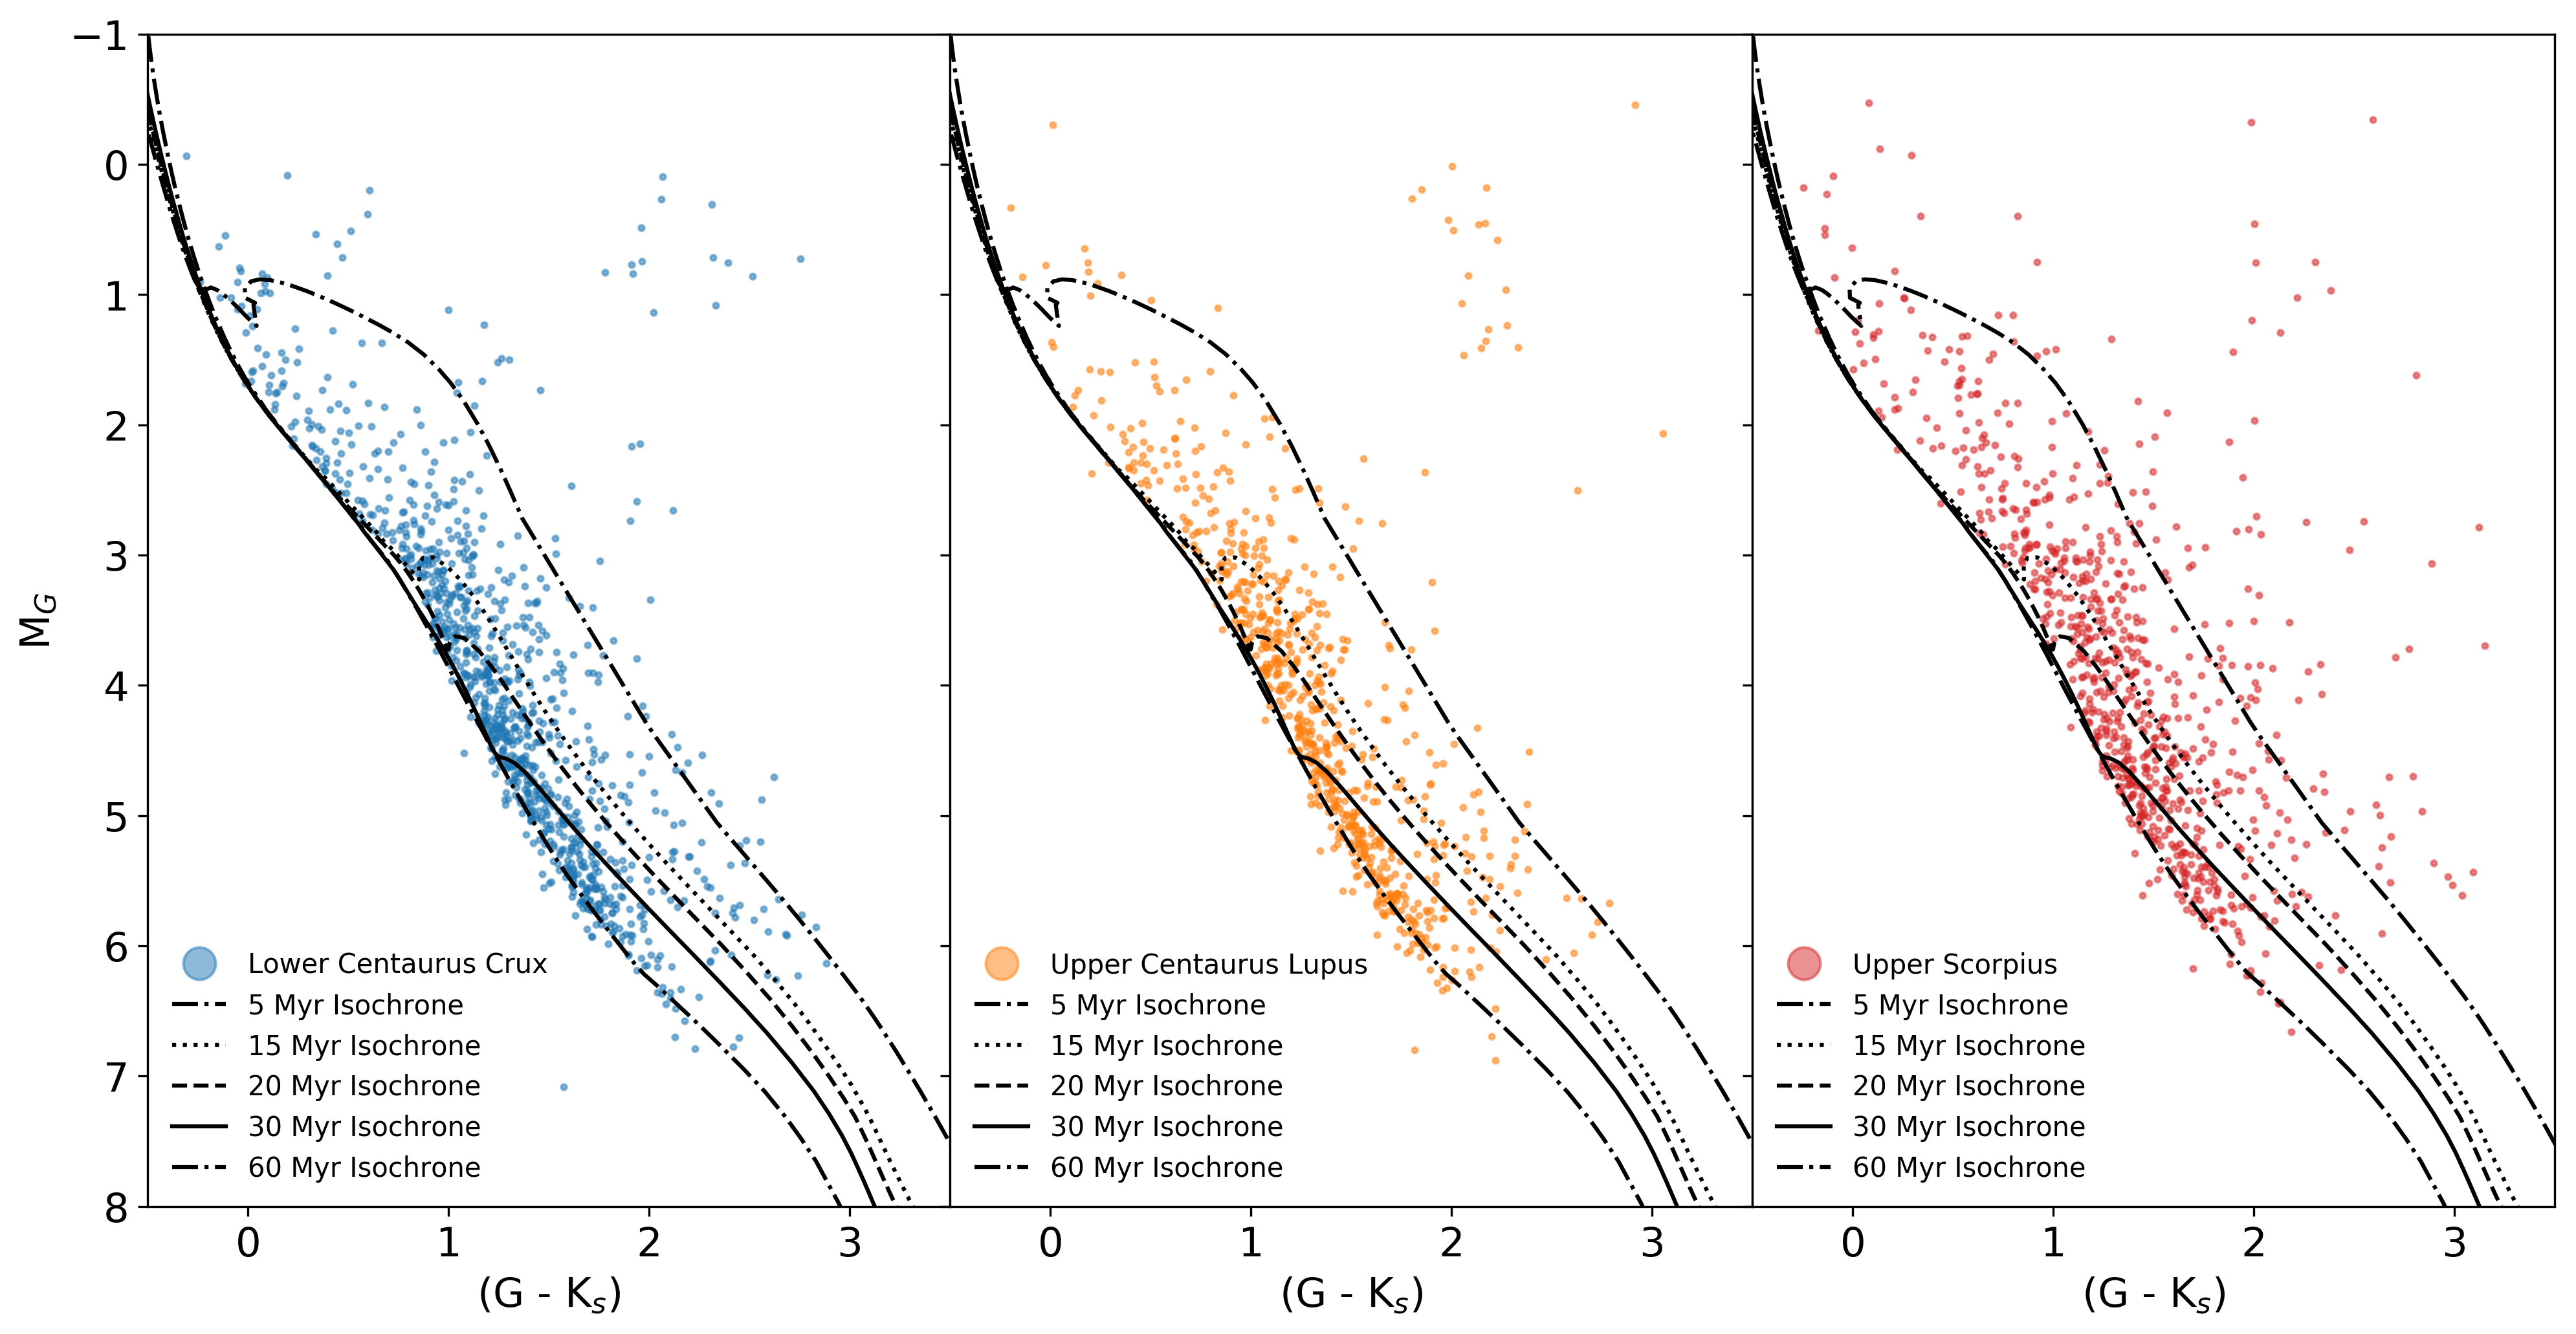
\includegraphics[width = 15cm, height = 8.5cm]{./Graficos/Capitulo_3/5_Sco-Cen/Mag_Col_diagram_3_Extintion_cut.png}} 
\caption{\scriptsize{Something!}}
\label{fig:Isochrones_1}
\end{figure}

\begin{figure}[!ht]
\centering
  \subfloat{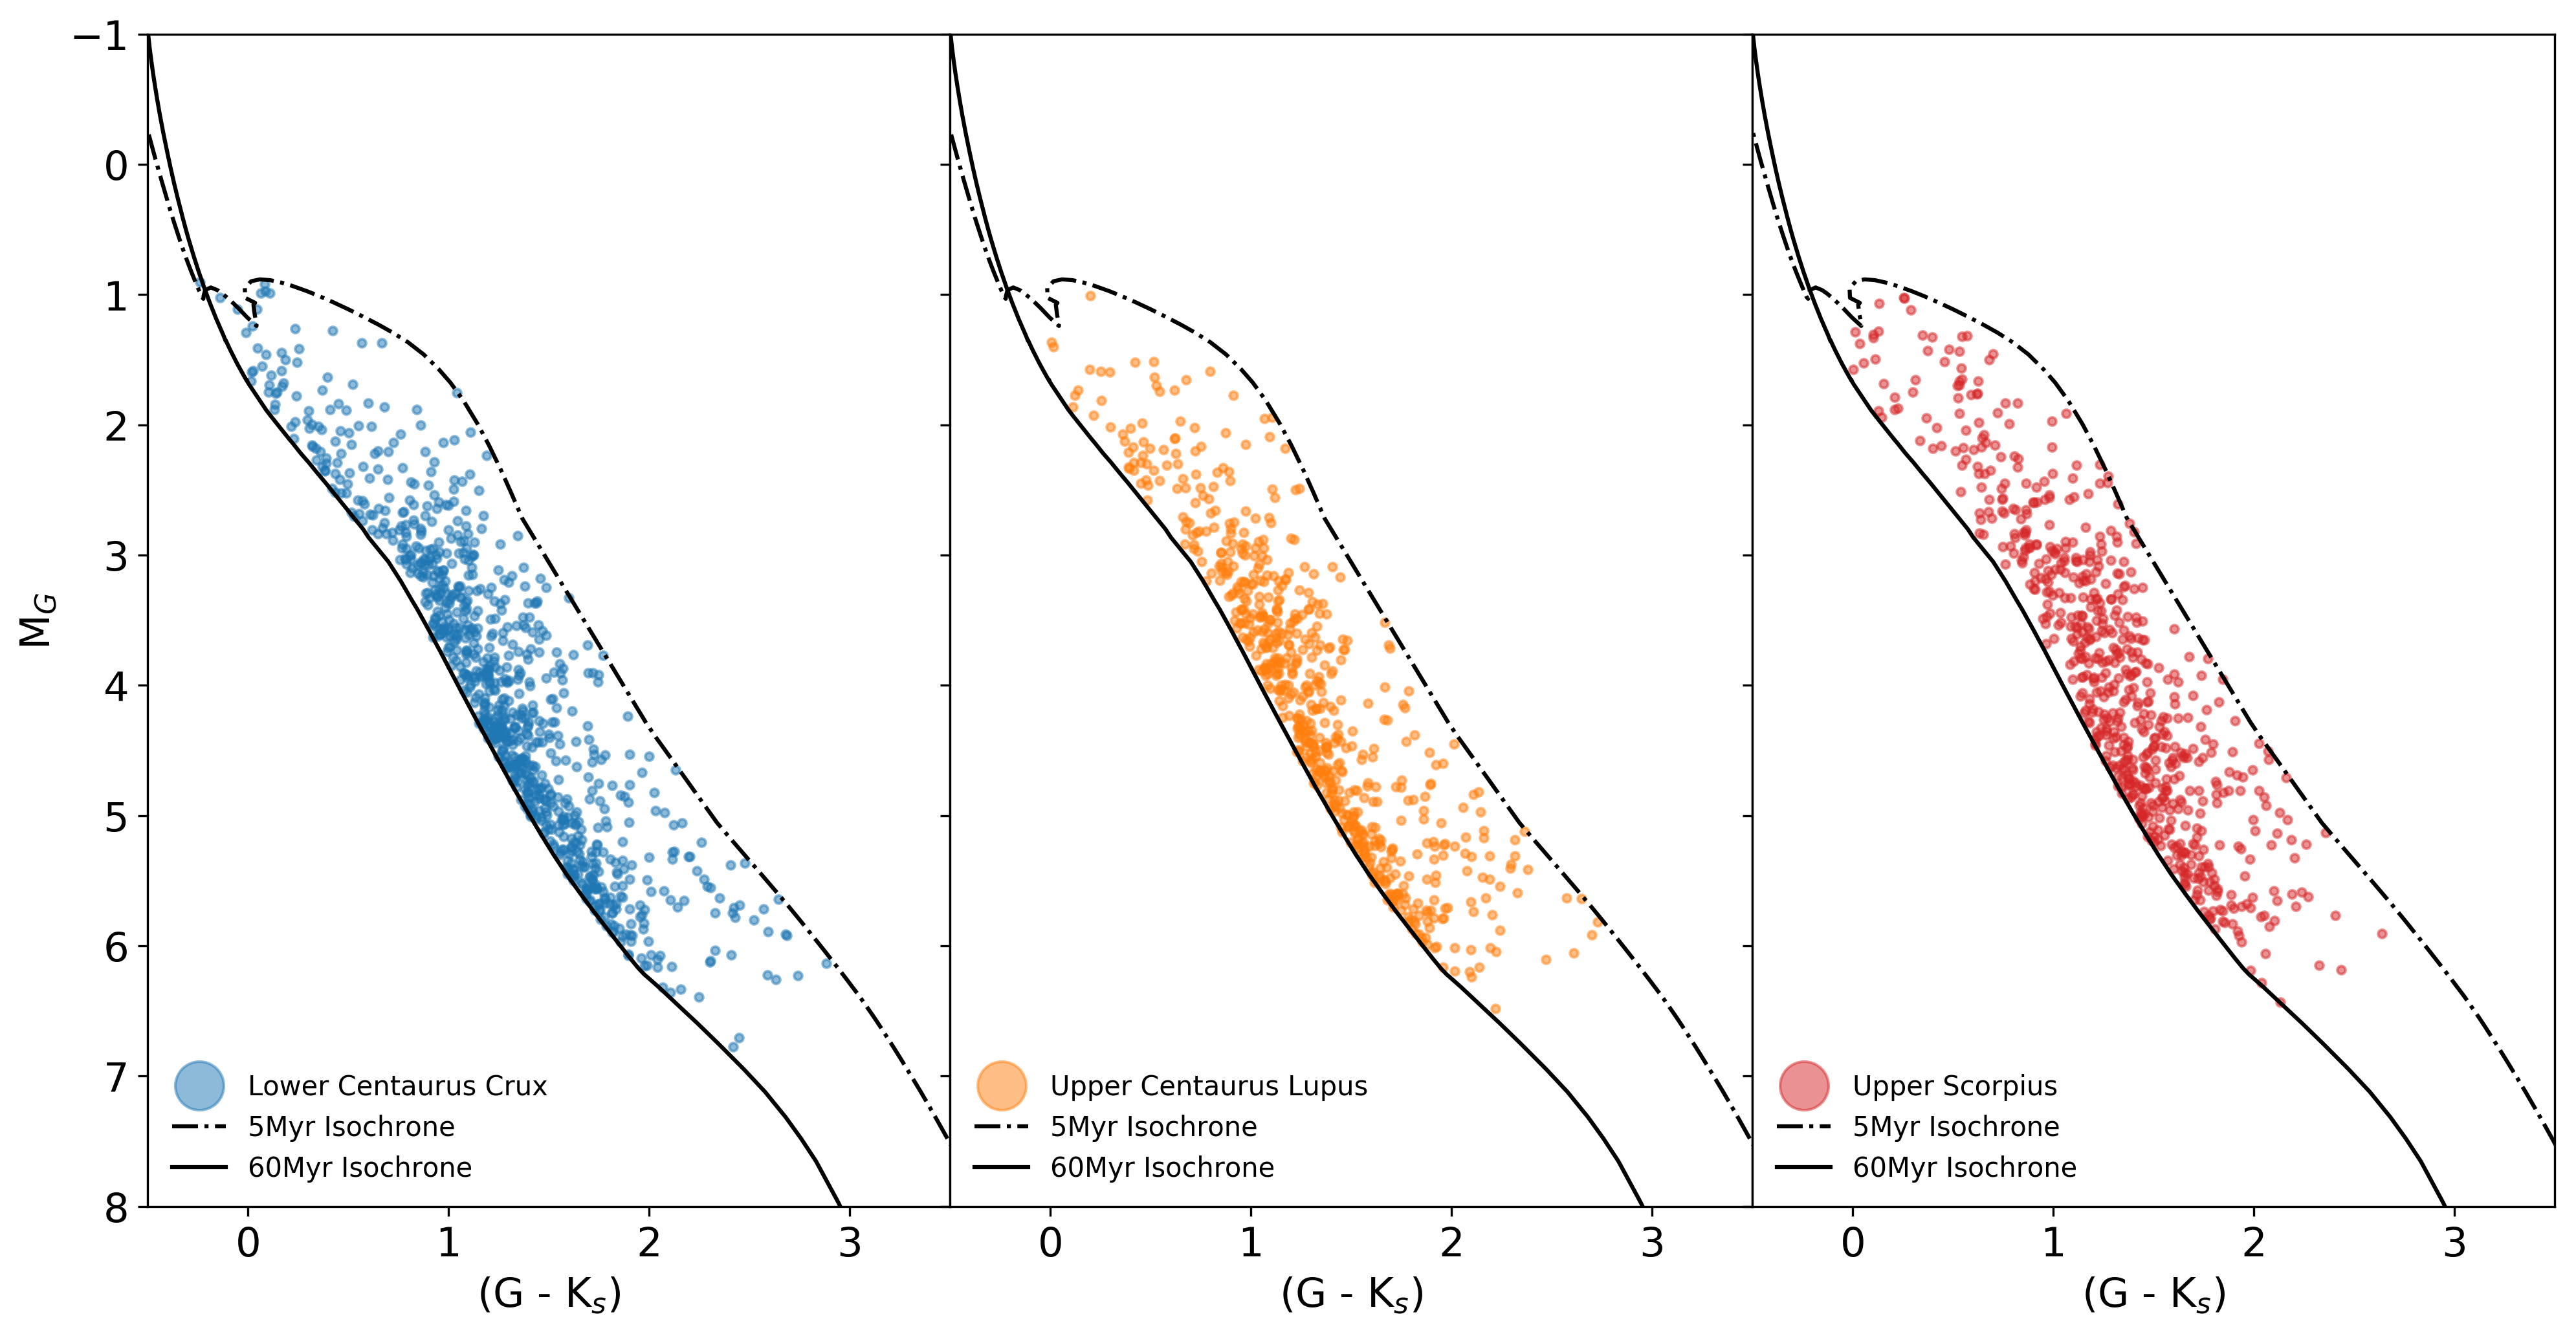
\includegraphics[width = 15cm, height = 8.5cm]{./Graficos/Capitulo_3/5_Sco-Cen/final_Sample_SCOCEN_Original.png}} 
\caption{\scriptsize{Something!}}
\label{fig:Isochrones_2}
\end{figure}

Besides this, if we want to obtain a reliable sample of star which belong to Sco-Cen, we need to include the extinction in each sub-region when computing the stellar tracks and isochrones. As can be seen from \autoref{fig:Isochrones_1}, the $60$-Myr gently touches the main-sequence of this association, thus, it seems legit to compute this isochrone with $\textnormal{A}_\textnormal{v} = 0$ because extinction will shift the isochrones upwards and we will lose stars lying on the main-sequence. However, in the case of the $5$-Myr isochrone, if we include extinction, then the isochrone will shift upwards including more stars that could be ruled out by our first selection method. Therefore, we proceed to compute the $5$-Myr isochrone including the extinction factor. Based on observation from \cauthor{1989A&A...216...44D}\citeyear{1989A&A...216...44D}, we were able to calculate the average, median and $90$-percentile extinction values for each sub-region. In the case of LCC a total number of 41 stars were used, while for UCL and US, 141 and 100 stars, respectively. In \autoref{fig:SCOCEN_Extinction}, the histograms for each sub-region are shown along with the average, median, and $90$-percentile extinction values. In the case of LCC and UCL, the values are always quite similar, but in the case of US, the values are significantly higher which may affect more drastically the isochrones and stellar tracks in comparison to the other two sub-regions. The values obtained for the average, are in agreement with values reported by \cauthor{2018MNRAS.tmp..210W}\citeyear{2018MNRAS.tmp..210W} and are well correlated with the distribution of the dust, as seen in the IRAS $100 \mu \textnormal{m}$ map \cauthor{1989A&A...216...44D}\citeyear{1989A&A...216...44D}. These values are $0.23$, $0.17$, $0.76$ for LCC, UCL, and US, repectively.\\     

\begin{figure}[!ht]
\centering
  \subfloat{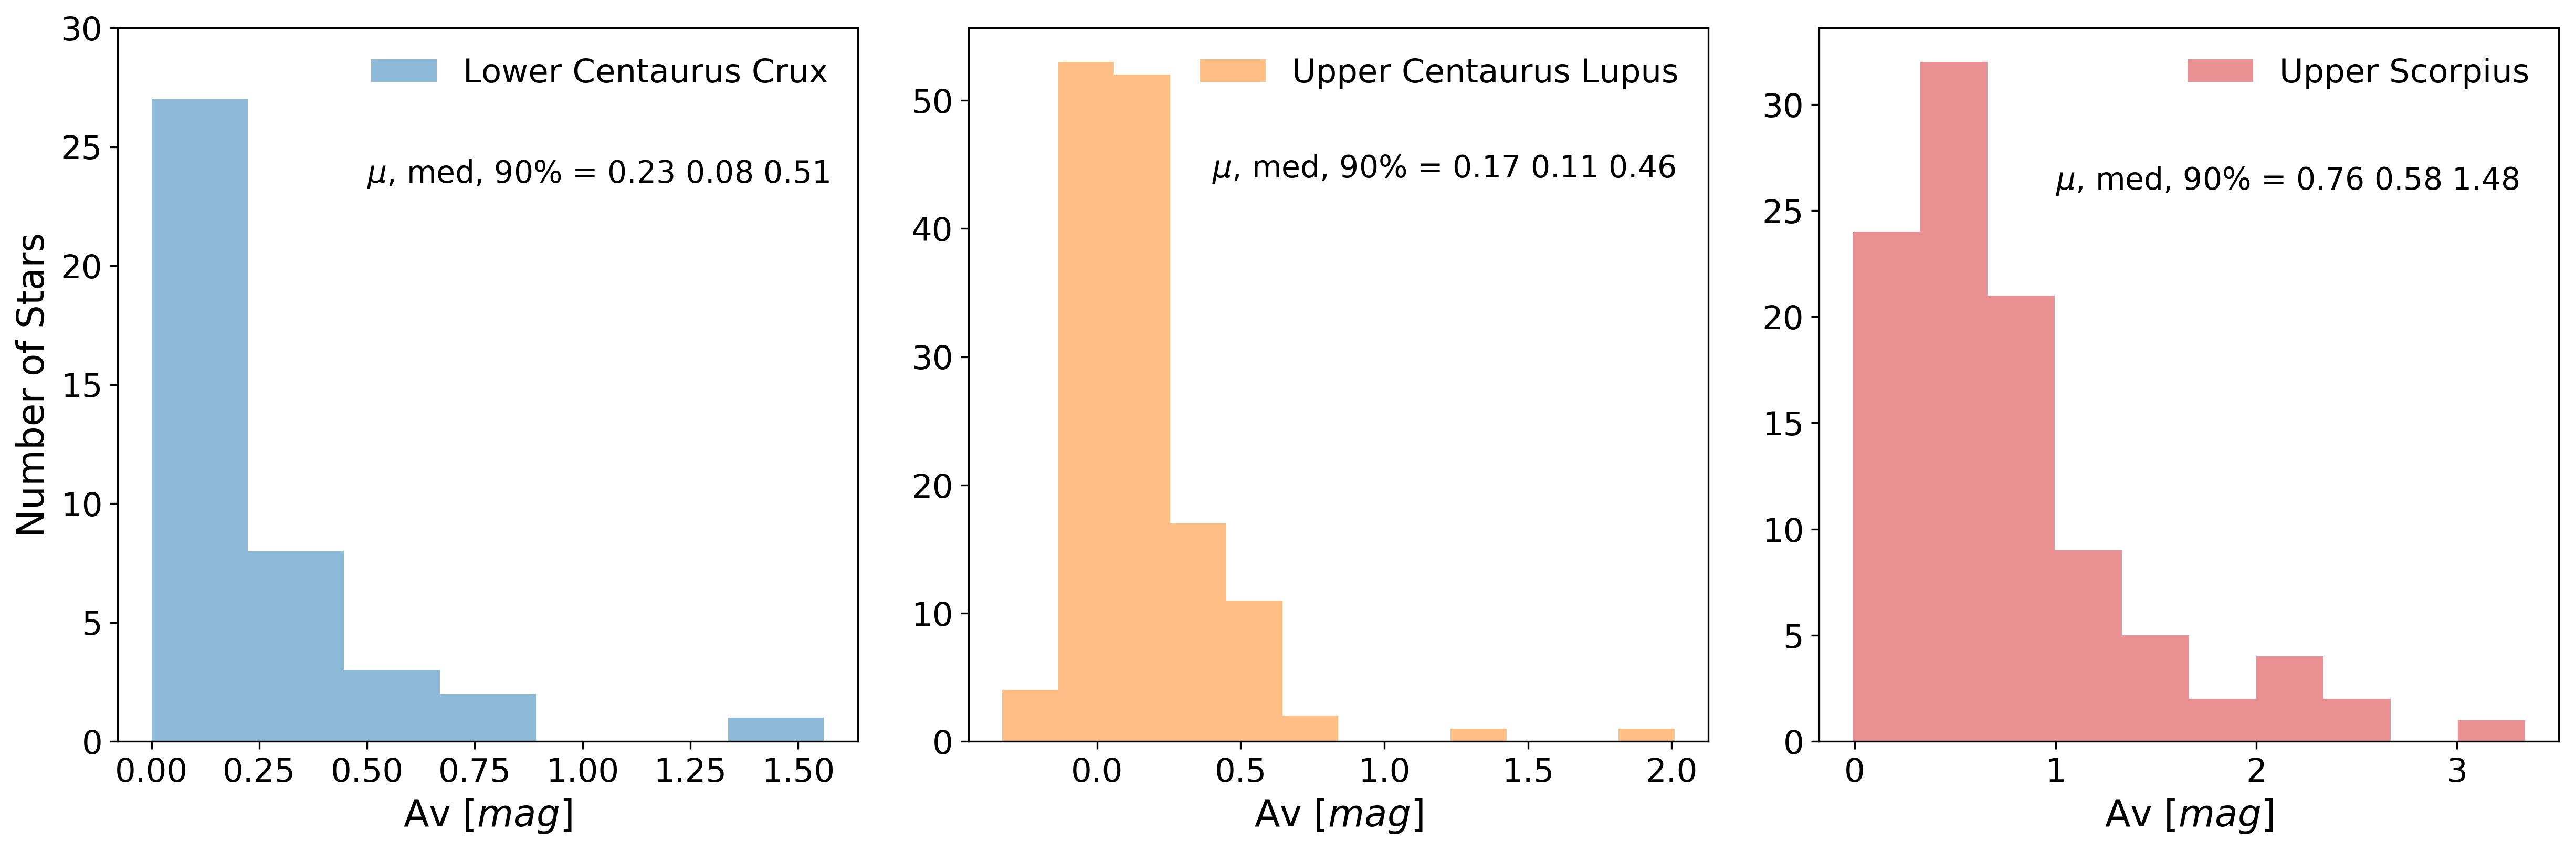
\includegraphics[width = 15.5cm, height = 5cm]{./Graficos/Capitulo_3/5_Sco-Cen/Av_histograms.png}} 
\caption{\scriptsize{Something!}}
\label{fig:SCOCEN_Extinction}
\end{figure}

On top of that, the $5$-Myr isochrone was computed using the average extinction values reported above to perform the selection of stars in the color-magnitude diagrams once more. As can be seen in \autoref{fig:Isochrones_3}, the shape of the $5$-Myr isochrone when introducing the extinction factor changes dramatically, moving upwards, increasing the number of stars in our selection. The same happens to LCC and UCL but in a less proportion. However, it is worth noting that the isochrones do not cross each other around $\textnormal{M}_\textnormal{G} \sim 1.0~[\textnormal{mag}]$ as was the case shown in \autoref{fig:Isochrones_1}, allowing for brighter stars to be selected in our sample. If we center our view in the stellar tracks, it is evident from \autoref{fig:Stellar_Tracks_3} that there exists a displacement downwards. However, as stars above $2.1 \textnormal{M}_\odot$ are not a lot, and this does not change that much, we will not perform any cut in stellar mass but we will just cut in stellar age using the isochrones. The new cut and final sample using the isochrones in which the youngest isochrone is affected by extinction is shown in \autoref{fig:Isochrones_4}.\\ 

\begin{figure}[!ht]
\centering
  \subfloat{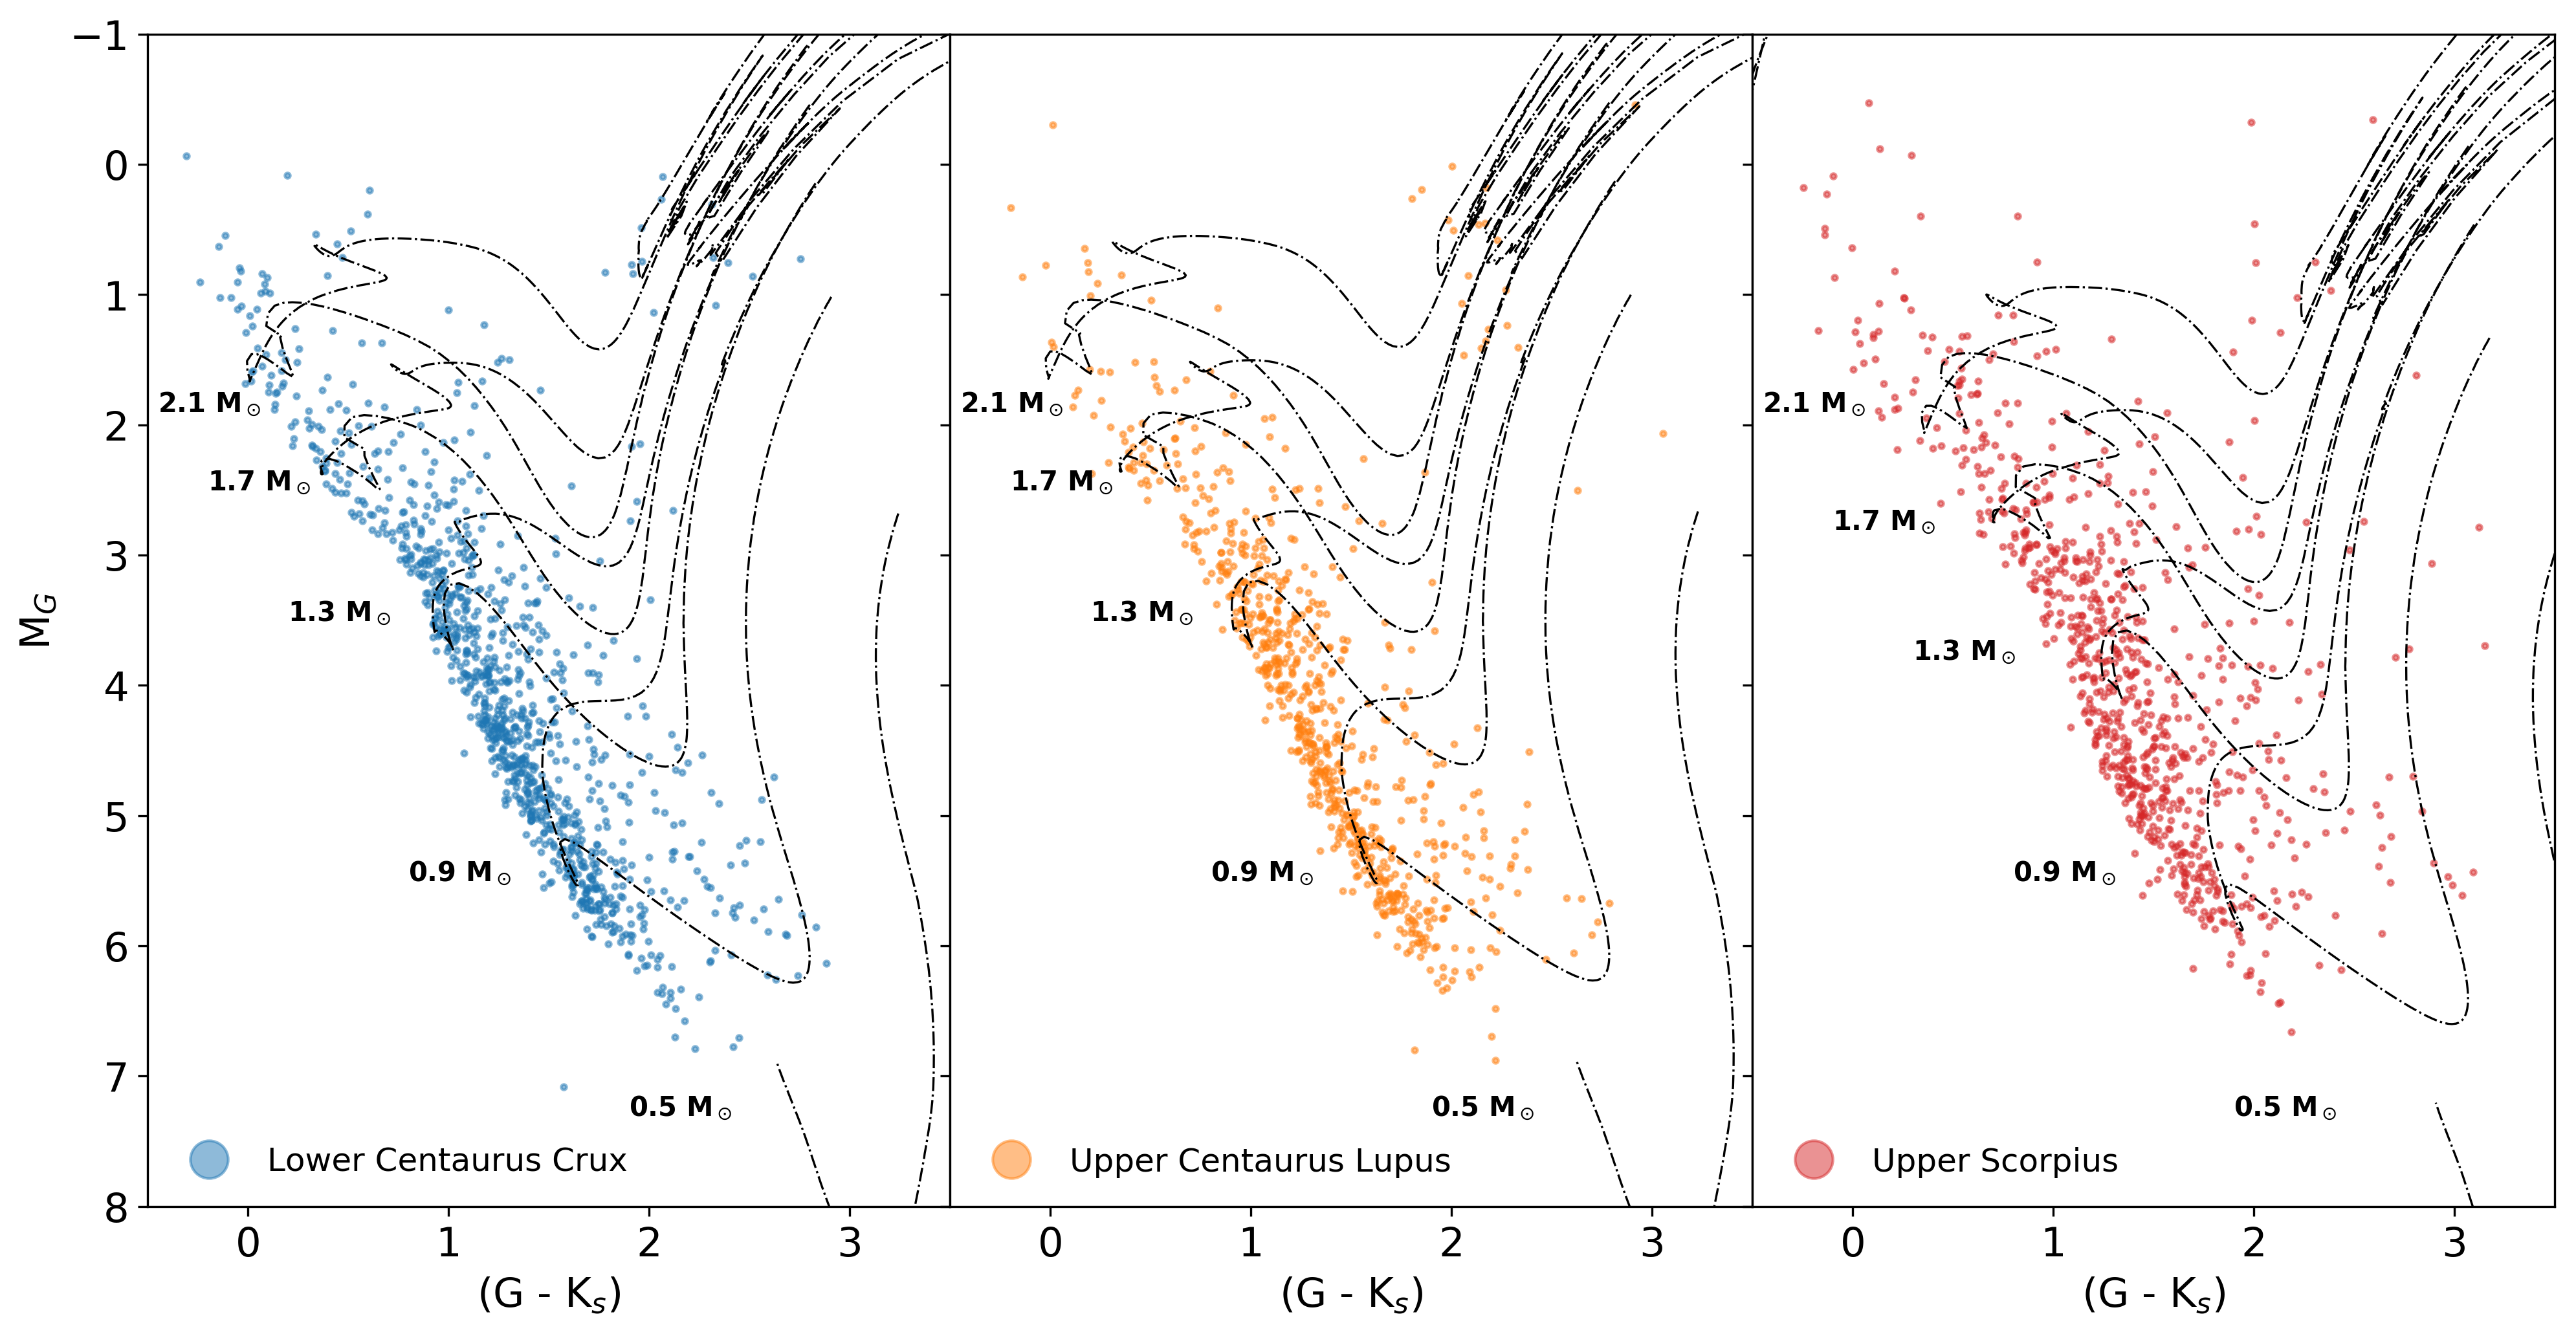
\includegraphics[width = 15cm, height = 8.5cm]{./Graficos/Capitulo_3/5_Sco-Cen/Mag_Col_diagram_4_Extintion_1.png}} 
\caption{\scriptsize{Something!}}
\label{fig:Stellar_Tracks_3}
\end{figure}

\begin{figure}[!ht]
\centering
  \subfloat{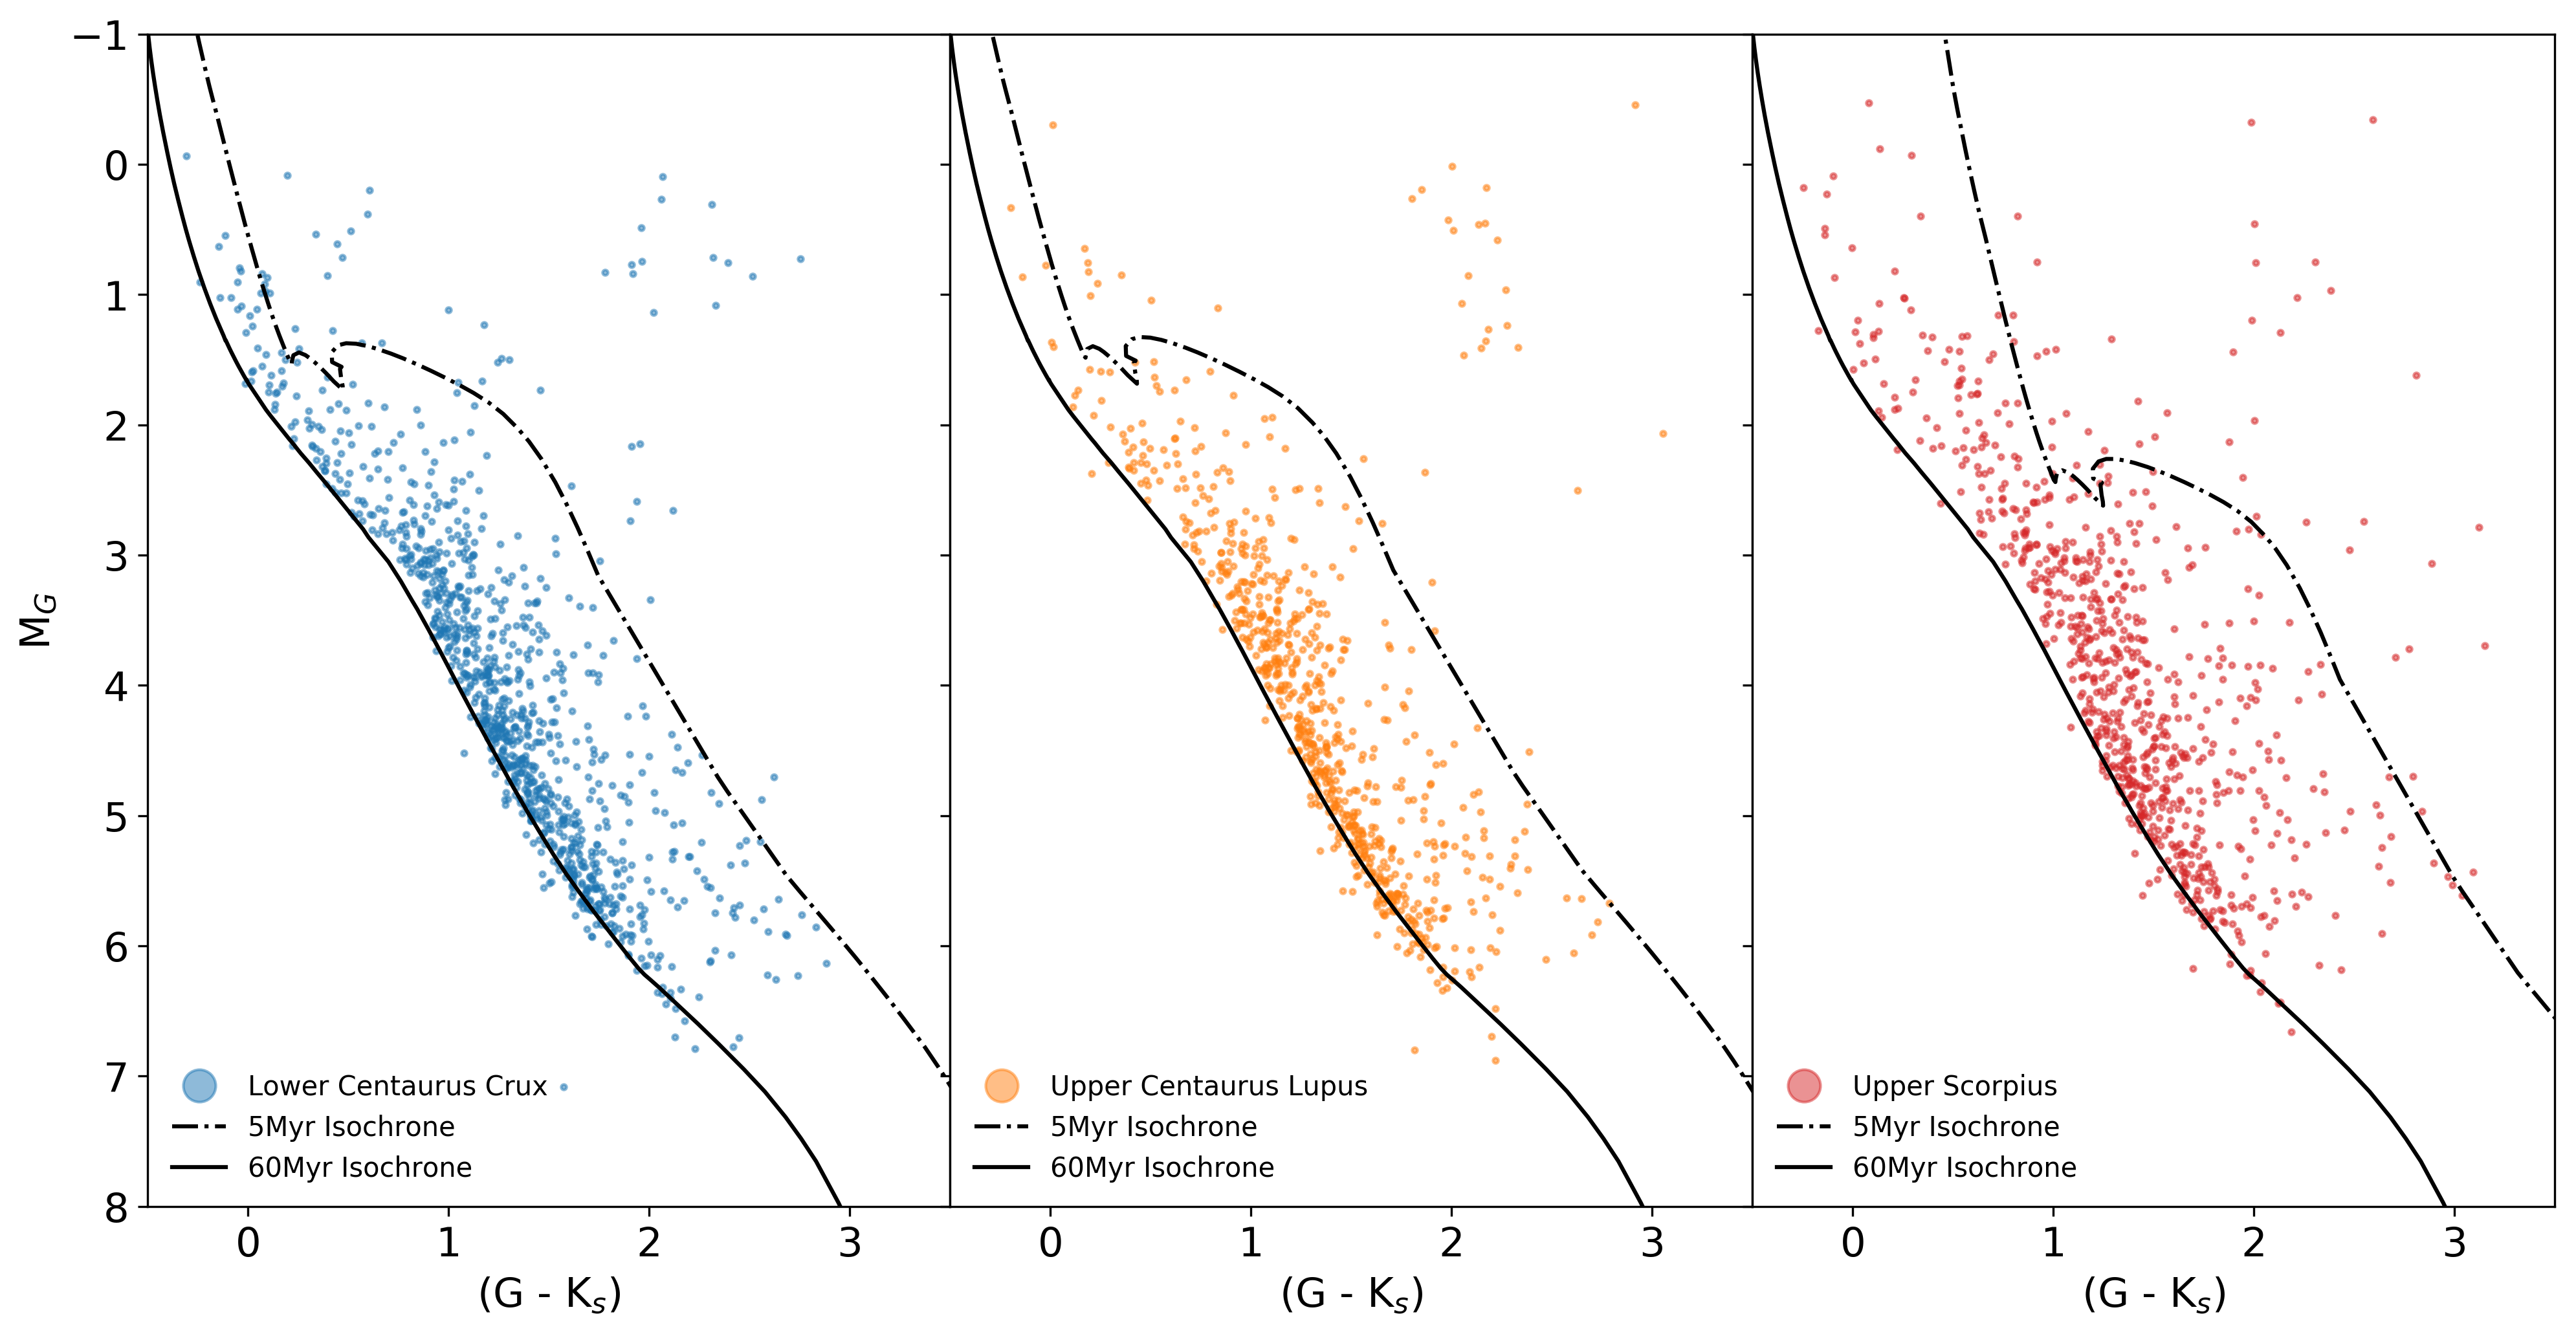
\includegraphics[width = 15cm, height = 8.5cm]{./Graficos/Capitulo_3/5_Sco-Cen/final_Sample_SCOCEN_2.png}} 
\caption{\scriptsize{Something!}}
\label{fig:Isochrones_3}
\end{figure}

\begin{figure}[!ht]
\centering
  \subfloat{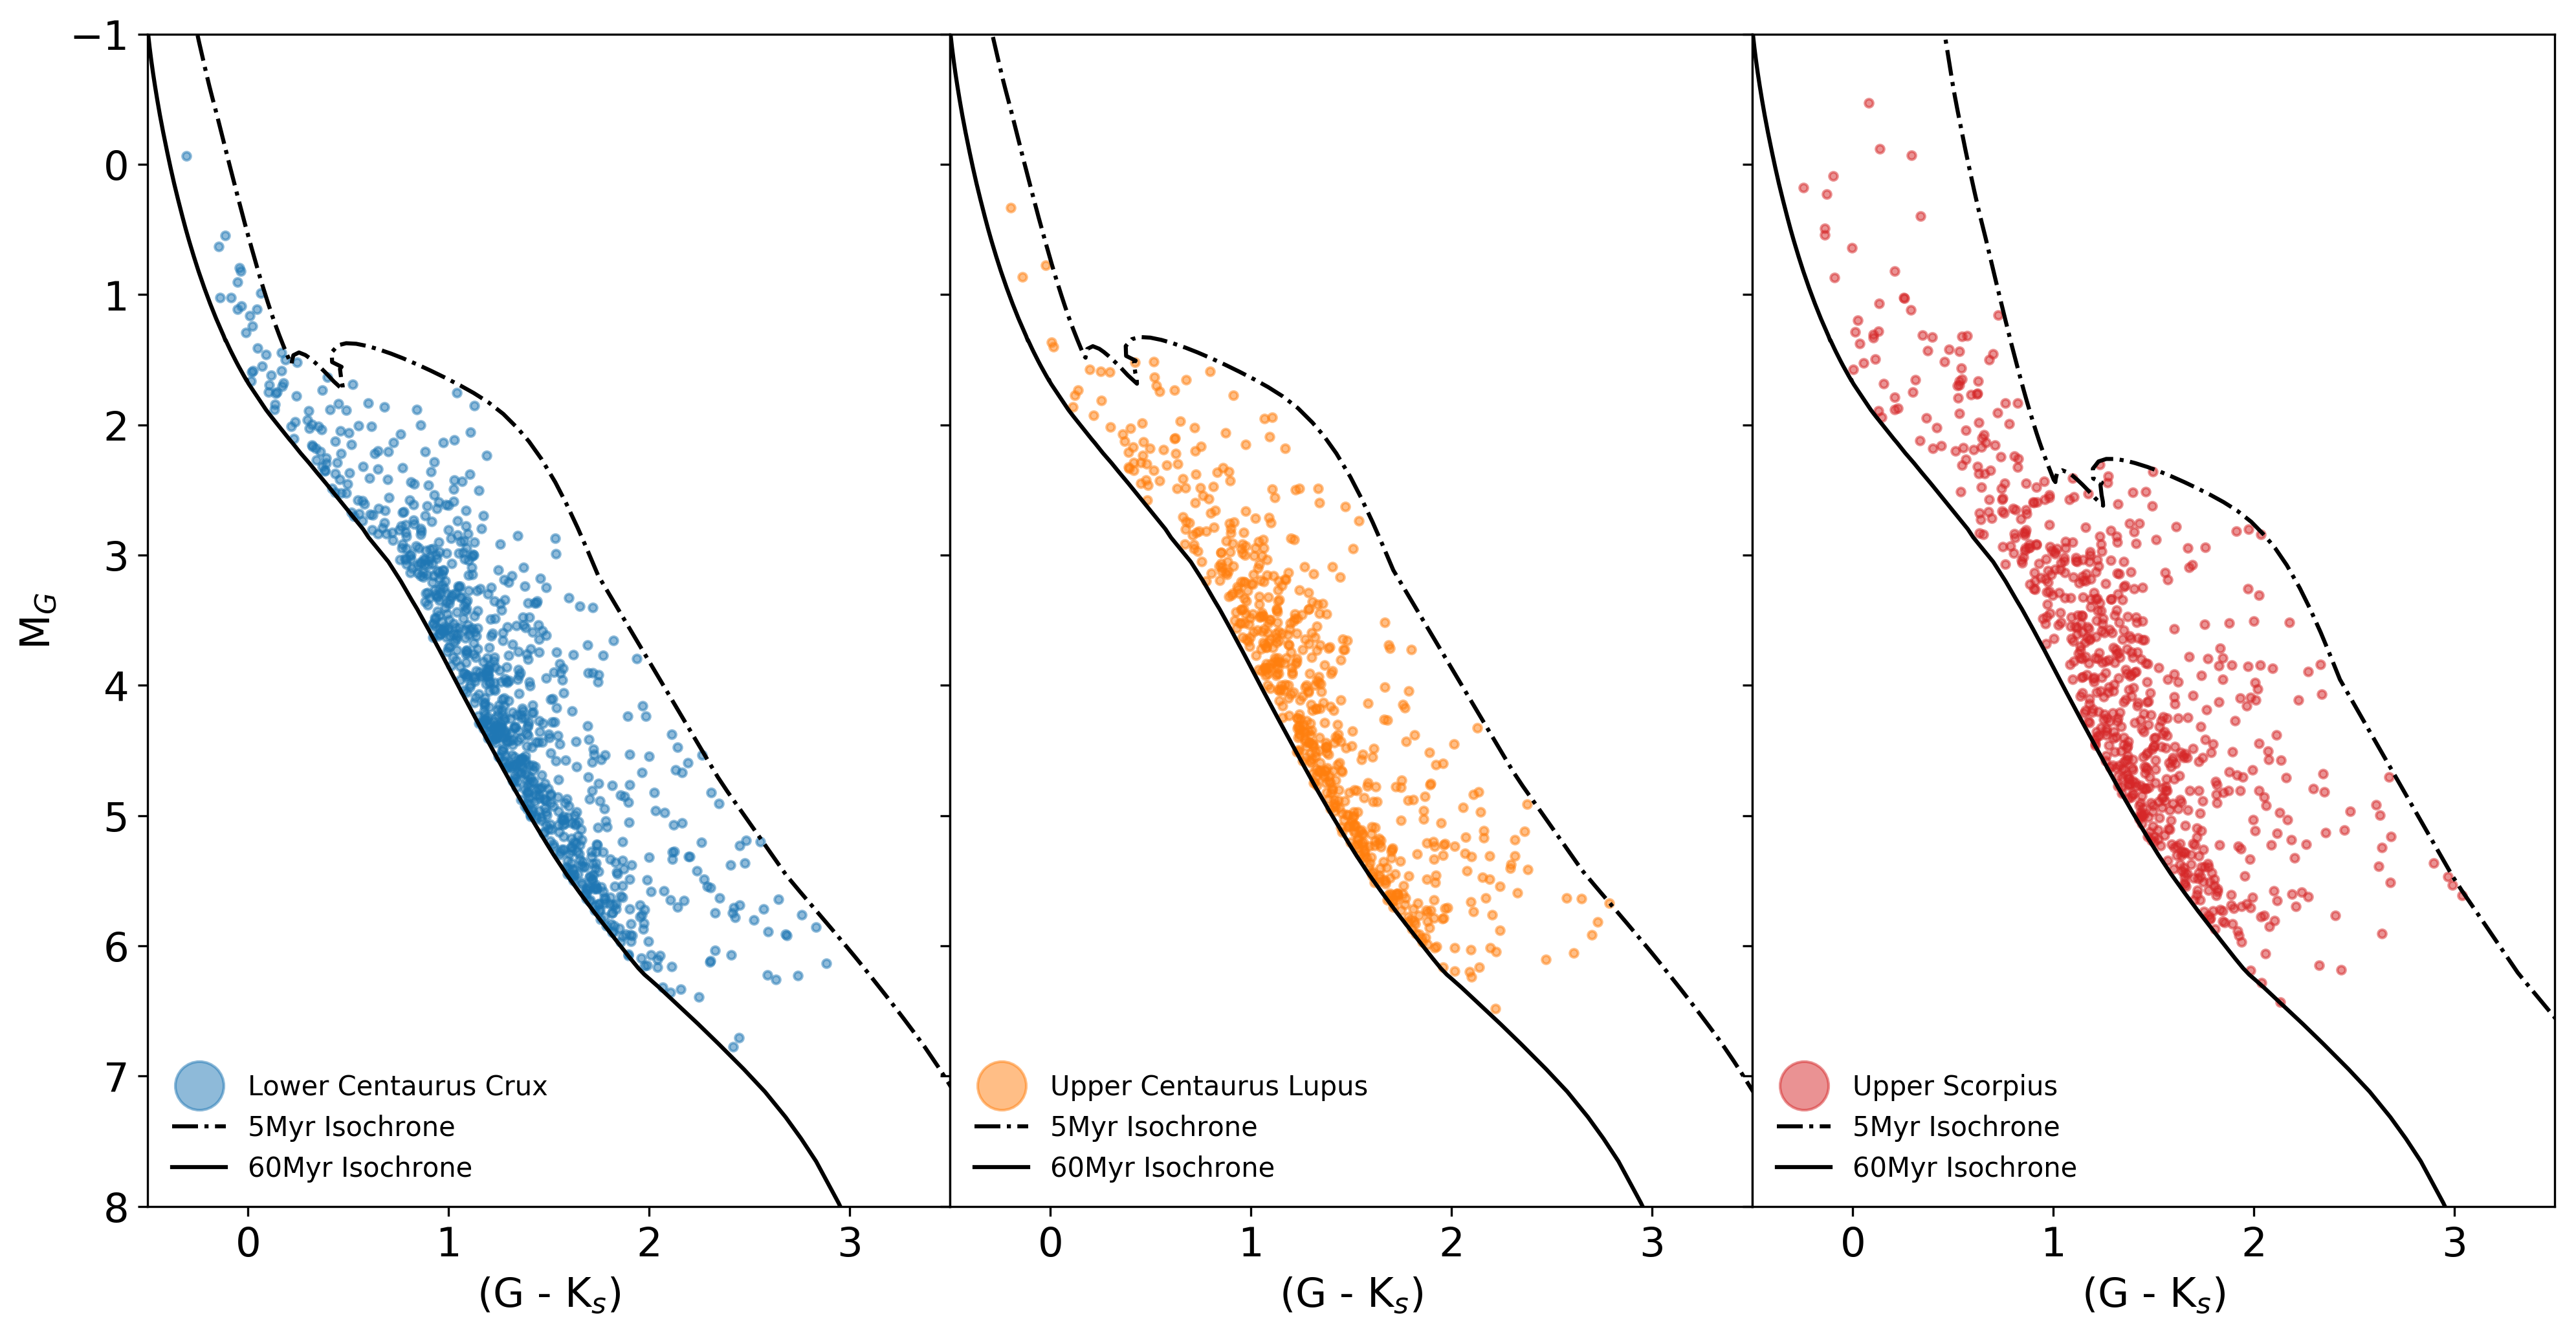
\includegraphics[width = 15cm, height = 8.5cm]{./Graficos/Capitulo_3/5_Sco-Cen/final_Sample_SCOCEN.png}} 
\caption{\scriptsize{Something!}}
\label{fig:Isochrones_4}
\end{figure}

The main goal out of this process is to obtain a reliable sample which contain as much as possible stars which could be potential candidates to belong to the Sco-Cen association based on distance and dynamical properties derived from literature. As was stated before, this analysis was performed on a sample data using \textit{Gaia}-DR1, and the final sample is made of LCC $= 889$, UCL $= 644$, and US $= 705$ stars respectively, in which there is a slight increase in the number of stars per sub-region compared to the case in which no extinction is use as expected because the region between the isochrones is now larger.\\

% Decir que esto se hace para obtener las coordenasdas que van a ser usadas en SuperWASP.
% Tengo que hablar sobre Gaia DR2, como cambiaron las cosas, como se hizo todo de nuevo y como cambiaron estos numeros y como van a ser usados en SuperWASP.
% Decir que se uso SuperWASP con DR1 pero el cmabio con DR2 no es mucho en algunos campos y en otros si, mirar los verdaderos numeros. 
% Decir que del DR2 sale la ultima muestra final que sera usada para hacer las curvas de luz. 

%============================================================================================================================================================

\section{Light Curves}

